% =============================================================================
% Target venue : ACM SIGSOFT FSE 2027
% Format       : ACM sigconf (acmart class)
% Purpose      : Final submission
% Backup       : paper_updated_backup_complex_2026_08_03.tex
% =============================================================================
\documentclass[sigconf,review,anonymous,balance=false]{acmart}

\acmConference{FSE '27}{July 12--16, 2027}{Shenzhen, China}
\acmDOI{}
\acmISBN{}
\setcopyright{acmlicensed}

\usepackage{amsmath}
\usepackage{graphicx}
\graphicspath{{figures/}}
\usepackage{booktabs}
\usepackage{array}
\usepackage{tabularx}
\usepackage{url}
\usepackage{xcolor}
\usepackage{tikz}
\usetikzlibrary{arrows.meta,positioning,shapes.geometric}

\newcolumntype{Y}{>{\raggedright\arraybackslash}X}

\title{Data-Flow Fault Observation for Agentic Microservices}

\author{Deepak Sunil Chavan}
\affiliation{%
  \institution{Concordia University}
  \department{Department of Electrical and Computer Engineering}
  \city{Montreal}
  \country{Canada}}
\email{deepaksunil.chavan@concordia.ca}

\begin{document}

\begin{abstract}
Agentic microservices combine LLM reasoning, tool calls, and conventional
service APIs. This makes failures harder to observe than in ordinary
microservices: a workflow may complete all steps while still passing a wrong
amount, product, recipient, or shipping decision to the next agent. This paper
uses LKW-style data-flow checkpoints and RIP analysis to expose these failures.
B1 records oracle checkpoint values, B2 characterizes no-fault variation, and
B3 activates one configured fault mode per run. We evaluate the method on agent
workflows from Google Online Boutique (GB) and RetailBen (RB). Across the two
complete ten-fault B3 configurations, the checkpoints exposed 51 of 58
conclusive faulty runs (87.9\%, Wilson 95\% CI [77.1, 94.0]\%); two runs were
inconclusive. The traces also identify the first infected agent, downstream
deviations, and whether a case is structurally detectable or requires semantic
inspection; two targeted chains separately test boundary containment. These
results show that checkpoint-level value comparison can
reveal semantic faults that successful workflow completion alone would miss.
\end{abstract}

\begin{CCSXML}
<ccs2012>
 <concept><concept_id>10011007.10011074.10011099</concept_id><concept_desc>Software and its engineering~Software testing and debugging</concept_desc><concept_significance>500</concept_significance></concept>
 <concept><concept_id>10010147.10010257</concept_id><concept_desc>Computing methodologies~Artificial intelligence</concept_desc><concept_significance>300</concept_significance></concept>
</ccs2012>
\end{CCSXML}
\ccsdesc[500]{Software and its engineering~Software testing and debugging}
\ccsdesc[300]{Computing methodologies~Artificial intelligence}

\keywords{agentic microservices, data-flow testing, fault injection, LKW, RIP,
LLM agents, human-in-the-loop}

\maketitle

% =============================================================================
\section{Introduction}
% =============================================================================

Modern microservice systems are increasingly being integrated with LLM agents.
Instead of calling a service directly, an agent may read a user task, choose a
tool, call a gRPC service, interpret the response, and pass a result to another
agent. This creates a new reliability problem. The service call may succeed,
the agent may return a plausible answer, and the workflow may continue, but a
business value may already be wrong.

For example, a payment agent may charge the wrong amount, a currency agent may
return a fabricated conversion, or a shipping agent may choose the wrong carrier
while still producing a valid-looking response. The same problem also appears in
catalog price manipulation, corrupted email bodies, empty or injected ad or
recommendation lists, and inventory or shipment mismatches. Step-level
monitoring is not enough for these failures because the workflow does not
necessarily crash. Detecting them requires evidence about the values crossing
agent and service boundaries.

This paper studies that problem using LKW data-flow checkpoints combined with
RIP analysis. LKW checkpoints observe selected variables at definition and use
points. RIP separates three questions: was the faulty code reached, did it
infect program state, and did that infection propagate to an observable output?
Together, they let us explain not only whether a fault was detected, but where
it first appeared and how far it travelled.

We evaluate the approach on GB e-commerce workflows and RB shipping workflows.
The experiment separates three roles: B1 supplies controlled oracle values, B2
measures normal variation, and B3 tests observability under one injected fault
per run. This separation prevents normal LLM variation from being mistaken for
a fault and supports RIP analysis of the resulting traces.

\textbf{Contributions.}
\begin{itemize}
  \item We define an LKW/RIP checkpoint method that selects business-critical
        variables and aligns agent checkpoints with service observation points.
  \item We provide a controlled B1/B2/B3 protocol that separates oracle values,
        normal variation, and single-fault traces.
  \item We evaluate ten fault types across GB and RB workflows and report
        run-level detection results with explicit denominators and confidence
        intervals.
  \item We use the traces to analyze first infection, propagation, HITL needs,
        boundary recovery, stability, and the current limits of attribution.
\end{itemize}

% =============================================================================
\section{Related Work}
% =============================================================================

\textbf{Data-flow testing.} Laski and Korel introduced data-flow oriented
testing, and Rapps and Weyuker formalized test selection using definitions and
uses of variables~\cite{lkw,rapps-weyuker}. We adapt this idea to agentic
microservices by selecting business-critical variables and observing their
definitions and uses at agent, tool, and service boundaries.

\textbf{Fault injection and chaos testing.} Microservice fault-injection work
often focuses on crashes, latency, network errors, and degraded service
responses~\cite{chaosengineering,microservicefi,istio}. Our work complements
this view by studying structural agent failures and semantic data corruption
that can remain hidden when a workflow completes.

\textbf{LLM agents and guardrails.} Agent benchmarks and tool-use frameworks
evaluate whether LLMs can call tools and complete tasks~\cite{react,agentbench,
toolbench,langgraph,autogen}. Guardrail work studies how to constrain unsafe
outputs~\cite{nemoguar,llmguardrails}. Our work focuses on the execution trace:
we ask whether the data passed between agents is correct at the moment it is
defined and used.

These research areas address related parts of the problem, but they do not by
themselves connect a known agent fault to the first corrupted business value
and its downstream propagation. Our method makes that connection by comparing
faulty checkpoint traces with an oracle and a no-fault variation envelope, then
interpreting the difference through RIP.

% =============================================================================
\section{Benchmarking Microservices and Agentification}
\label{sec:benchmarks}
% =============================================================================

We study three workflow surfaces across two domains: Google Online Boutique
(GB) checkout, RetailBen (RB) shipping quote, and RB ship order. GB is based on
an external cloud-native microservice benchmark, whereas RB is a two-agent
LangGraph shipping workflow constructed for this study. Each surface has an
LLM-facing agent, an experiment helper or service adapter, and a microservice
interface. In the systematic experiments, the helpers invoke Ollama for agent
decisions and use controlled mock clients for service responses. They are
controlled experimental boundaries, not evidence that every call reached a
deployed service. LKW checkpoints record values at the agent--helper and
helper--service-interface boundaries.

Figure~\ref{fig:architecture-simple} abstracts the common experimental pattern;
it is not a claim that GB and RB share one deployed call graph. The agent boxes
represent LLM-facing agents whose decisions can vary across runs. B1 is
deterministic only in the narrower sense that it uses controlled helpers and
fixed service responses; this does not make the LLM agent or a deployed service
deterministic.

\subsection{System Architecture Design}

The evaluation architecture separates variable LLM reasoning from controlled
service interaction. Each workflow has four conceptual components: a task entry
point, an LLM agent that plans and chooses tools, a controlled helper that
translates the decision into a service-interface call, and the microservice
interface represented by a mock client in the systematic runs. This separation
lets us observe business values where they are created and consumed rather than
only at the final task outcome.

The agent layer may vary across runs because it performs reasoning and tool
selection, while controlled helper inputs and service responses make the task
replayable. LKW checkpoints are placed at the agent--adapter and
adapter--service-interface boundaries. Values such as amount, currency,
carrier, tracking ID, and recipient can be corrupted at these boundaries even
when the workflow completes. The architecture therefore supports both fault
localization and observation of silent data-flow errors.

\begin{figure*}[t]
\centering
\resizebox{0.92\textwidth}{!}{%
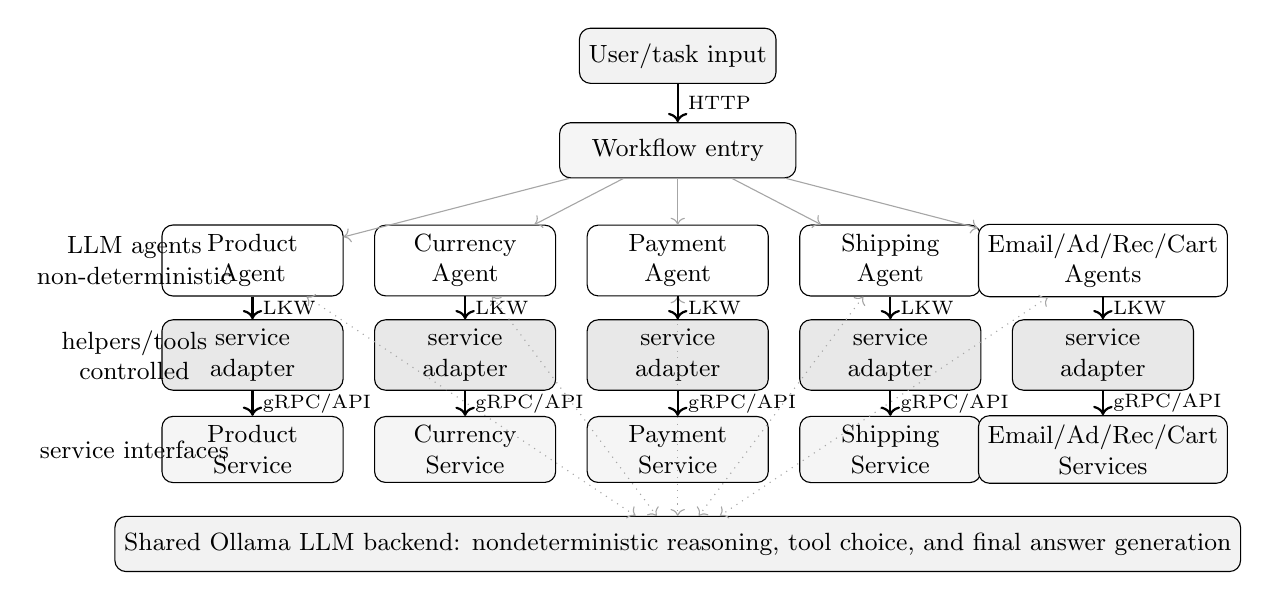
\begin{tikzpicture}[
      box/.style={draw,rounded corners,align=center,minimum height=0.7cm},
      svc/.style={box,fill=gray!8,minimum width=2.3cm},
      agt/.style={box,fill=white,minimum width=2.3cm},
      adapt/.style={box,fill=gray!18,minimum width=2.3cm},
      llm/.style={box,fill=gray!10,minimum width=13.8cm},
      every node/.style={font=\small}
]
\node[box,fill=gray!10,minimum width=2.2cm] (front) at (0,3.2) {User/task input};
\node[svc,minimum width=3.0cm] (checkout) at (0,2.0) {Workflow entry};
\node[agt] (a1) at (-5.4,0.6) {Product\\Agent};
\node[agt] (a2) at (-2.7,0.6) {Currency\\Agent};
\node[agt] (a3) at (0,0.6) {Payment\\Agent};
\node[agt] (a4) at (2.7,0.6) {Shipping\\Agent};
\node[agt] (a5) at (5.4,0.6) {Email/Ad/Rec/Cart\\Agents};
\node[adapt] (t1) at (-5.4,-0.6) {service\\adapter};
\node[adapt] (t2) at (-2.7,-0.6) {service\\adapter};
\node[adapt] (t3) at (0,-0.6) {service\\adapter};
\node[adapt] (t4) at (2.7,-0.6) {service\\adapter};
\node[adapt] (t5) at (5.4,-0.6) {service\\adapter};
\node[svc] (s1) at (-5.4,-1.8) {Product\\Service};
\node[svc] (s2) at (-2.7,-1.8) {Currency\\Service};
\node[svc] (s3) at (0,-1.8) {Payment\\Service};
\node[svc] (s4) at (2.7,-1.8) {Shipping\\Service};
\node[svc] (s5) at (5.4,-1.8) {Email/Ad/Rec/Cart\\Services};
\node[llm] (llm) at (0,-3.0) {Shared Ollama LLM backend: nondeterministic reasoning, tool choice, and final answer generation};

\draw[->,thick] (front) -- node[right,font=\scriptsize] {HTTP} (checkout);
\foreach \agent in {a1,a2,a3,a4,a5} {
      \draw[->,gray!70] (checkout) -- (\agent);
      \draw[<->,dotted,gray!70] (\agent) -- (llm);
}
\foreach \agent/\tool/\service in {a1/t1/s1,a2/t2/s2,a3/t3/s3,a4/t4/s4,a5/t5/s5} {
      \draw[->,thick] (\agent) -- node[right,font=\scriptsize] {LKW} (\tool);
      \draw[->,thick] (\tool) -- node[right,font=\scriptsize] {gRPC/API} (\service);
}
\node[align=center,font=\small] at (-6.9,0.6) {LLM agents\\non-deterministic};
\node[align=center,font=\small] at (-6.9,-0.6) {helpers/tools\\controlled};
\node[align=center,font=\small] at (-6.9,-1.8) {service interfaces};
\end{tikzpicture}}
\caption{Common experimental architecture for the GB and RB workflows. Agent
groups use a shared Ollama backend, while controlled helpers and mock clients
represent service interaction in the systematic runs. LKW checkpoints record
business values at agent--helper and helper--service-interface boundaries. The
figure abstracts the two benchmarks rather than depicting one deployed call
graph.}
\Description{Conceptual architecture connecting task input to grouped GB and RB agents, controlled service adapters, service interfaces, and a shared Ollama backend. LKW checkpoints observe each agent-to-adapter boundary.}
\label{fig:architecture-simple}
\end{figure*}

\subsection{Google Online Boutique Checkout (GB)}

Google Online Boutique (GB) is an open-source cloud-native e-commerce
microservice benchmark~\cite{google-ob}. We add LLM-facing agents to seven
service surfaces: product catalog, currency, payment, email, recommendation,
advertising, and cart. Each agent selects a service tool through a controlled
helper. ProductCatalogAgent, CurrencyAgent, PaymentAgent, and EmailServiceAgent
participate in the complete systematic B3 matrix; RecommendationAgent,
AdServiceAgent, and CartAgent provide isolated evidence.

The GB faults cover wrong products or prices, incorrect currency conversion,
payment-amount tampering, corrupted email content, and invalid advertising or
recommendation output. These failures may preserve the expected sequence of
steps while corrupting values used by downstream services.

\subsection{RetailBen Shipping Quote (RB)}

RetailBen (RB) is a two-agent LangGraph shipping workflow constructed for this
study. ShippingQuoteAgent receives package, destination, and inventory context
and returns a carrier, price quote, and delivery window. Its checkpoints expose
whether inventory, carrier, quote, or delivery information changes before the
result is passed downstream.

\subsection{RetailBen Ship Order (RB)}

ShipOrderAgent receives the approved quote and order details, selects a carrier,
creates a tracking record, saves the order, and evaluates escalation conditions.
Because it consumes the upstream quote, the workflow reveals whether an error
is blocked, corrected, or propagated into order state.

\begin{table}[t]
\centering
\caption{Benchmarked agent domains. GB and RB are kept separate throughout the
paper to avoid mixing domain-specific failure behavior.}
\label{tab:domains}
\begin{tabularx}{\columnwidth}{lYY}
\toprule
\textbf{Domain} & \textbf{Agents} & \textbf{Typical failures} \\
\midrule
GB & Product, currency, payment, email, cart, recommendation, ad
   & Price, amount, ID, recipient, routing, and content corruption \\
RB & Shipping quote, ship order
   & Carrier, quote, tracking, escalation, and delivery-policy errors \\
\bottomrule
\end{tabularx}
\end{table}

\begin{table*}[t]
\centering
\caption{Evidence coverage by agent role. ``Isolated'' denotes a local fault
harness or result artifact; ``Systematic'' denotes participation in the
workflow runner; ``B3-10'' denotes participation in the complete ten-fault
matrix reported in Table~\ref{tab:b3-headline-simple}. The checkout
orchestrator has structural RIP checks but no field-level B1 oracle. ``HITL''
means the role appears in the saved per-fault HITL classification artifact; it
does not mean that every fault requires human intervention.}
\label{tab:service-coverage-simple}
\footnotesize
\begin{tabularx}{\textwidth}{lcccccY}
\toprule
\textbf{Service/agent} & \textbf{Domain} & \textbf{Isolated} & \textbf{Systematic} & \textbf{B3-10} & \textbf{HITL} & \textbf{Measured role} \\
\midrule
PaymentAgent          & GB & yes & yes & yes & yes & Amount tampering; Chain A sink \\
CurrencyAgent         & GB & yes & yes & yes & yes & Rate manipulation; Chain A source \\
EmailServiceAgent     & GB & yes & yes & yes & yes & Corrupted body \\
ProductCatalogAgent   & GB & yes & yes & yes & yes & Price manipulation; Chain B source \\
CheckoutOrchestrator  & GB & yes & yes & yes & no  & Workflow coordination; structural RIP only \\
RecommendationAgent  & GB & yes & no  & no  & yes & Isolated faults; Chain B sink \\
AdServiceAgent        & GB & yes & no  & no  & yes & Isolated ad faults \\
CartAgent             & GB & yes & no  & no  & no  & Isolated C\# harness/artifacts \\
ShipOrderAgent        & RB & yes & yes & yes & no  & Shipment loss in systematic B3 \\
ShippingQuoteAgent    & RB & yes & yes & yes & no  & Inventory mismatch in systematic B3 \\
\bottomrule
\end{tabularx}
\end{table*}

% =============================================================================
\section{Framework Definition and Design}
\label{sec:framework}
% =============================================================================

The framework is a four-phase procedure for testing an agentified service
workflow. It defines the observation boundary, selects business-critical
variables, activates one configured fault mode, and compares the resulting trace with
no-fault evidence. The phases are summarized across
Figures~\ref{fig:architecture-simple}, \ref{fig:fault-injection-simple},
and~\ref{fig:testing-protocol-simple}.

\textbf{Phase 1: Agentification boundary definition.} We first identify the
service workflow being studied and separate three roles: nondeterministic LLM
agents, controlled experiment helpers/tools, and service interfaces. This
prevents a common ambiguity: controlled replay does not imply that either the
LLM or a deployed service is deterministic. LKW checkpoints are placed at this
agent--helper and helper--service-interface boundary.

\textbf{Phase 2: Guarded-variable and checkpoint design.} For each benchmark,
we select the business variables that determine correctness: amount, currency,
product ID, carrier, quote, tracking ID, email body, recommendation list, and
similar values. A variable becomes guarded only if it drives a business decision,
crosses an agent--adapter or adapter--service boundary, and can be corrupted
without necessarily crashing the workflow.

\textbf{Phase 3: Controlled fault injection.} We activate exactly one fault
mode per B3 run. The four general FM modes are applied across the workflow;
each business-specific BL mode is targeted to its owning agent. A mode may
remove a step, change routing, fabricate an output, or tamper with a business
value. This design gives each run one configured cause while preserving the
intended global or targeted injection scope.

\textbf{Phase 4: Oracle comparison and RIP interpretation.} B1 provides the
fault-free checkpoint oracle. B2 characterizes no-fault behavior in isolated
repetitions and, separately, in the live-LLM systematic runner. B3 runs the same
task with one injected fault. A fault is detected only when B3 deviates from B1
beyond the B2 equivalence relation. RIP then explains whether the fault was
reached, infected checkpoint state, and propagated to a downstream agent or
business output.

We use the following vocabulary throughout the paper. A \emph{benchmark task}
is one GB or RB workflow instance. An \emph{agentified service} is a service
accessed through an LLM-facing agent and a controlled helper/tool. A
\emph{guarded variable} is a business value selected for LKW observation. An
\emph{LKW checkpoint} is a named definition or use point where that variable is
recorded. A \emph{fault mode} is a controlled perturbation applied during B3.
An \emph{infection checkpoint} is the first recorded point whose value or
required-step status violates its fixed B1/B2 comparison relation. It can be
unlocalized when an expected checkpoint is absent and no earlier corrupted
value was recorded.

% =============================================================================
\section{LKW and RIP Checkpoint Design}
\label{sec:lkw-rip}
% =============================================================================

This section links LKW data-flow testing, controlled fault injection, and the
resulting fault-observability measurements.

The benchmark first determines the business variables that must remain correct.
LKW identifies where those variables are defined and used, and fault injection
perturbs one selected variable or decision. Detection occurs when B3 loses a
required checkpoint or records a value outside the relation established by B1
and B2. RIP then identifies where the deviation first appears and whether it
reaches a later observation.

\subsection{What an LKW Checkpoint Records}

An LKW checkpoint is a named observation point inside an agent or at an agent
boundary. It records the step, selected business values, and, when available,
diagnostic fields when a guarded variable is defined or used. Useful
checkpoints occur when a task enters an agent, before or after a tool call, and
before the final answer. Diagnostic fault flags are test-harness evidence; they
are not assumed to exist in production monitoring.

We select an LKW variable only when it satisfies three criteria. First, it must
drive a business decision in the benchmark workflow. Second, it must cross an
agent--adapter or adapter--service boundary. Third, an injected fault must be
able to corrupt it without necessarily crashing the workflow. Table~\ref{tab:lkw-variable-criteria}
shows this selection rule for the studied agents.

\begin{table*}[t]
\centering
\caption{LKW guarded-variable selection criteria. The variables are chosen from
benchmark semantics, not from arbitrary trace fields. Each guarded variable is
important because a wrong value can still allow the workflow to complete while
changing the business outcome.}
\label{tab:lkw-variable-criteria}
\footnotesize
\begin{tabularx}{\textwidth}{l l Y Y}
\toprule
\textbf{Domain} & \textbf{Agent} & \textbf{Guarded LKW variables} & \textbf{Why these variables are selected} \\
\midrule
GB & ProductCatalogAgent & action, product-ID set, count, price-change flag & These fields identify wrong routing, missing or fabricated products, and price manipulation before downstream use. \\
GB & CurrencyAgent & input units, target currency, converted units, currency-swap flag & These fields reveal whether the requested conversion or its returned amount changed. \\
GB & PaymentAgent & requested/charged amount, validation and tamper flags, transaction ID, save state & These fields show whether validation ran, the amount remained correct, and the transaction was valid and saved. \\
GB & EmailServiceAgent & recipient, email type, body length, send status & These fields expose wrong recipients or templates, truncated content, and skipped delivery. \\
GB & RecommendationAgent & user context, recommendation count, hallucination/injection flags & These fields expose empty, fabricated, or injected recommendation output. \\
GB & AdServiceAgent & context-key set, ad count, hallucination flag & These fields expose wrong context, empty or duplicated output, and fabricated ads. \\
GB & CartAgent & user/product ID, quantity, item count, success state & These isolated-harness fields show whether the expected basket item is added and returned. \\
RB & ShippingQuoteAgent & item count, quoted cost & These fields expose inventory inflation and quote corruption before order creation. \\
RB & ShipOrderAgent & carrier, stale-quote flag, tracking ID, escalation and save state & These fields show whether the quote becomes a valid, persisted order or requires intervention. \\
\bottomrule
\end{tabularx}
\end{table*}

\begin{table}[t]
\centering
\caption{Logical schema of a raw LKW checkpoint record. Agent identity may be
stored by the enclosing per-agent trace, while guarded values and diagnostic
metadata are stored in the checkpoint data object.}
\label{tab:lkw-schema}
\begin{tabularx}{\columnwidth}{lY}
\toprule
\textbf{Field} & \textbf{Meaning} \\
\midrule
Agent & GB or RB role that owns the enclosing trace \\
Step & Named point such as \texttt{TASK\_START} or \texttt{CHARGE\_DONE} \\
Timestamp & Time recorded by the raw LKW producer \\
Data & Guarded runtime fields such as amount, product IDs, carrier, or body length \\
Diagnostic metadata & Optional experiment fields such as configured mode or harness flags \\
\bottomrule
\end{tabularx}
\end{table}

\begin{table*}[t]
\centering
\caption{Explicit alignment between agent-side LKW checkpoints and
service-interface observation points. B1 supplies expected values and B2
characterizes acceptable no-fault variation for these comparisons.}
\label{tab:checkpoint-alignment}
\footnotesize
\begin{tabularx}{\textwidth}{l l Y Y}
\toprule
\textbf{Domain} & \textbf{Agent checkpoint} & \textbf{Microservice observation point} & \textbf{Comparison relation} \\
\midrule
GB & \texttt{PaymentAgent: CHARGE\_DONE}
      & PaymentService request/response values (charged amount, transaction outcome)
      & Numeric tolerance ($\delta_{\epsilon}$) on amount + flag conformance ($\Sigma$) \\
GB & \texttt{CurrencyAgent: CONVERT\_DONE}
      & CurrencyService request/response values (source, target, converted amount)
      & Numeric tolerance ($\delta_{\epsilon}$) \\
GB & \texttt{ProductCatalogAgent: CATALOG\_DONE}
      & ProductCatalogService response values (product IDs, prices, list contents)
      & Set/schema equality ($\mathcal{S}$) + numeric tolerance ($\delta_{\epsilon}$) \\
GB & \texttt{EmailServiceAgent: EMAIL\_GENERATED/EMAIL\_SENT}
      & EmailService request/response values (recipient, content fields, send status)
      & Schema equality ($\mathcal{S}$) + flag conformance ($\Sigma$) \\
GB & \texttt{RecommendationAgent: RECOMMEND\_DONE}
      & RecommendationService request/response values (context IDs, recommendation IDs)
      & Set/schema equality ($\mathcal{S}$) \\
GB & \texttt{AdServiceAgent: ADS\_FETCHED}
      & AdService request/response values (context fields, ad IDs/URLs)
      & Set/schema equality ($\mathcal{S}$) \\
GB & \texttt{CartAgent: CART\_DONE}
      & CartService response values (item IDs, quantities, presence)
      & Set/schema equality ($\mathcal{S}$) + numeric tolerance ($\delta_{\epsilon}$) \\
RB & \texttt{ShippingQuoteAgent: QUOTE\_DONE}
      & Shipping quote service request/response values (inventory status, carrier, quote, ETA)
      & Numeric tolerance ($\delta_{\epsilon}$) + schema equality ($\mathcal{S}$) \\
RB & \texttt{ShipOrderAgent: CARRIER\_DONE/TRACKING\_DONE/SAVE\_DONE}
      & Ship-order service request/response values (carrier, tracking ID, save status, escalation)
      & Schema equality ($\mathcal{S}$) + flag conformance ($\Sigma$) \\
\bottomrule
\end{tabularx}
\end{table*}

The checkpoint-equivalence relations in Tables~\ref{tab:checkpoint-alignment}
and~\ref{tab:fault-lkw-ckpt} are declared before the B3 campaign using B1
semantics and B2 no-fault observations. B3 is then evaluated under these fixed
relations so calibration and evaluation remain separated.

Table~\ref{tab:fault-lkw-ckpt} summarizes the field-level instrumentation map
for the Python service-facing agents. It is a design table, not a results table.
The checkout orchestrator is evaluated structurally through expected-step
checks, and CartAgent has isolated harness evidence but is not part of this
field-level map. The table shows where each listed fault should become visible,
the LKW criterion and use type, and the comparison class applied to B3.

\begin{table*}[t]
\centering
\caption{Mapping faults to LKW criteria and checkpoints. Agents marked
\textbf{(RB)} are from RetailBen; all other agents are from Google Boutique.
\textbf{Infect. checkpoint} is the first LKW point where the injected fault is
expected to become observable. \textbf{AU} = All-Uses; \textbf{ADP} =
All-DU-Paths. \textbf{C-use} means computational use and \textbf{P-use} means
predicate/decision use. \textbf{Cmp.} groups the concrete B1/B3 checks:
$\delta_{\epsilon}$ = numeric exact, tolerance, or range check;
$\mathcal{S}$ = string, set, schema, or required-step conformance; and
$\Sigma$ = boolean or diagnostic-flag conformance.}
\label{tab:fault-lkw-ckpt}
\footnotesize
\setlength{\tabcolsep}{3pt}
\resizebox{\textwidth}{!}{%
\begin{tabular}{p{2.8cm}p{3.0cm}p{2.9cm}lll}
\toprule
\textbf{Agent} & \textbf{Fault mode} & \textbf{Infect. checkpoint} & \textbf{Criterion} & \textbf{Use} & \textbf{Cmp.} \\
\midrule
ShippingQuoteAgent \textbf{(RB)} & \texttt{BL-INV-MISMATCH} & \texttt{TASK\_START} & \textbf{AU/ADP} & C-use/P-use & $\delta_{\epsilon}$ \\
 & \texttt{BL-REFUND} & \texttt{QUOTE\_DONE} & \textbf{ADP} & C-use/P-use & $\delta_{\epsilon}$ \\
 & \texttt{FM-2.5} & \texttt{QUOTE\_DONE} & \textbf{ADP} & C-use/P-use & $\delta_{\epsilon}$ \\
\midrule
ShipOrderAgent \textbf{(RB)} & \texttt{BL-ESCALATION} & \texttt{ESCALATION\_CHECK} & \textbf{AU} & P-use & $\Sigma$ \\
 & \texttt{BL-SHIP-LOST} & \texttt{SAVE\_DONE} & \textbf{ADP} & C-use/P-use & $\mathcal{S}$ \\
 & \texttt{BL-VENDOR} & \texttt{CARRIER\_DONE} & \textbf{AU} & C-use & $\mathcal{S}$ \\
 & \texttt{FM-1.2} & \texttt{TRACKING\_DONE} & \textbf{AU} & C-use & $\mathcal{S}$ \\
 & \texttt{FM-2.2} & \texttt{CARRIER\_DONE} & \textbf{AU} & C-use & $\mathcal{S}$ \\
 & \texttt{FM-2.5} & \texttt{CARRIER\_DONE} & \textbf{AU} & P-use & $\Sigma$ \\
 & \texttt{FM-3.1} & \texttt{TRACKING\_DONE} & \textbf{AU} & C-use & $\mathcal{S}$ \\
\midrule
PaymentAgent & \texttt{BL-AMOUNT-TAMPER} & \texttt{CARD\_VALIDATED} & \textbf{AU/ADP} & C-use/P-use & $\delta_{\epsilon}$ \\
 & \texttt{BL-DOUBLE-CHARGE} & \texttt{SAVE\_DONE} & \textbf{AU} & P-use & $\Sigma$ \\
 & \texttt{BL-TXN-LOST} & \texttt{SAVE\_DONE} & \textbf{AU} & P-use & $\Sigma$ \\
 & \texttt{FM-1.2} & \texttt{CARD\_VALIDATED} & \textbf{AU} & P-use & $\Sigma$ \\
 & \texttt{FM-2.2} & \texttt{CHARGE\_DONE} & \textbf{AU} & C-use/P-use & $\Sigma$ \\
 & \texttt{FM-2.5} & \texttt{CARD\_VALIDATED} & \textbf{AU/ADP} & C-use/P-use & $\delta_{\epsilon}$ \\
\midrule
CurrencyAgent & \texttt{BL-CONV-OVERFLOW} & \texttt{CONVERT\_DONE} & \textbf{AU} & C-use & $\delta_{\epsilon}$ \\
 & \texttt{BL-RATE-MANIP} & \texttt{CONVERT\_DONE} & \textbf{AU} & C-use & $\delta_{\epsilon}$ \\
 & \texttt{BL-STALE-RATE} & \texttt{CONVERT\_DONE} & \textbf{AU} & C-use & $\delta_{\epsilon}$ \\
 & \texttt{FM-1.2} & \texttt{CONVERT\_DONE} & \textbf{AU} & C-use/P-use & $\Sigma$ \\
 & \texttt{FM-2.2} & \texttt{CONVERT\_DONE} & \textbf{AU} & C-use & $\delta_{\epsilon}$ \\
 & \texttt{FM-2.5} & \texttt{CONVERT\_DONE} & \textbf{AU} & C-use & $\delta_{\epsilon}$ \\
\midrule
EmailServiceAgent & \texttt{BL-CORRUPT-BODY} & \texttt{EMAIL\_GENERATED} & \textbf{AU} & C-use & $\delta_{\epsilon}$ \\
 & \texttt{BL-SEND-SKIP} & \texttt{EMAIL\_SENT} & \textbf{AU} & C-use/P-use & $\Sigma$ \\
 & \texttt{FM-1.2} & \texttt{EMAIL\_GENERATED} & \textbf{AU} & C-use/P-use & $\Sigma$ \\
 & \texttt{FM-2.2} & \texttt{EMAIL\_GENERATED} & \textbf{AU} & P-use & $\Sigma$ \\
 & \texttt{FM-2.5} & \texttt{EMAIL\_GENERATED} & \textbf{AU} & C-use & $\Sigma$ \\
\midrule
ProductCatalogAgent & \texttt{BL-DUP-PRODUCT} & \texttt{CATALOG\_DONE} & \textbf{AU} & C-use/P-use & $\delta_{\epsilon}$ \\
 & \texttt{BL-PRICE-MANIP} & \texttt{CATALOG\_DONE} & \textbf{ADP} & C-use & $\Sigma$ \\
 & \texttt{BL-PROD-MISSING} & \texttt{CATALOG\_DONE} & \textbf{AU} & C-use/P-use & $\delta_{\epsilon}$ \\
 & \texttt{FM-1.2} & \texttt{CATALOG\_DONE} & \textbf{AU} & P-use & $\Sigma$ \\
 & \texttt{FM-2.2} & \texttt{CATALOG\_DONE} & \textbf{AU} & C-use/P-use & $\delta_{\epsilon}$ \\
\midrule
RecommendationAgent & \texttt{BL-EMPTY-RECS} & \texttt{RECOMMEND\_DONE} & \textbf{AU} & C-use/P-use & $\delta_{\epsilon}$ \\
 & \texttt{BL-INJECT-RECS} & \texttt{RECOMMEND\_DONE} & \textbf{AU} & P-use & $\Sigma$ \\
 & \texttt{FM-2.2} & \texttt{RECOMMEND\_DONE} & \textbf{AU} & C-use & $\Sigma$ \\
 & \texttt{FM-2.5} & \texttt{RECOMMEND\_DONE} & \textbf{AU} & C-use & $\Sigma$ \\
 & \texttt{FM-3.1} & \texttt{RECOMMEND\_DONE} & \textbf{AU} & C-use/P-use & $\delta_{\epsilon}$ \\
\midrule
AdServiceAgent & \texttt{BL-AD-INJECTION} & \texttt{ADS\_FETCHED} & \textbf{AU} & C-use/P-use & $\delta_{\epsilon}$ \\
 & \texttt{BL-DUP-ADS} & \texttt{ADS\_FETCHED} & \textbf{AU} & C-use/P-use & $\delta_{\epsilon}$ \\
 & \texttt{BL-EMPTY-ADS} & \texttt{ADS\_FETCHED} & \textbf{AU} & C-use/P-use & $\delta_{\epsilon}$ \\
 & \texttt{FM-1.2} & \texttt{CONTEXT\_EXTRACTED} & \textbf{AU} & C-use & $\mathcal{S}$ \\
 & \texttt{FM-2.2} & \texttt{ADS\_FETCHED} & \textbf{AU} & C-use & $\Sigma$ \\
 & \texttt{FM-2.5} & \texttt{CONTEXT\_EXTRACTED} & \textbf{AU} & C-use & $\mathcal{S}$ \\
\bottomrule
\end{tabular}}
\end{table*}

\subsection{B1, B2, and B3 Roles}

The experimental design uses three roles:

\begin{description}
  \item[B1: oracle.] Field-level B1 values are assembled from deterministic
            \texttt{NONE}-mode runs for six service agents. Shipping uses the
        selected no-fault systematic baseline. The checkout orchestrator has an
        expected step sequence but no field-level B1 oracle. B1 therefore
        defines the expected checkpoint state without claiming that all agents
        or deployed services are deterministic.
  \item[B2: no-fault characterization.] B2 contains three no-fault repetitions
        for seven surfaces: six deterministic agents use
        \texttt{use\_llm=false}, while the shipping surface uses the live LLM.
        A separate systematic B2 runner exercises the complete live-LLM
        workflow. Equivalence uses numeric, categorical, schema, set, or boolean
        relations instead of requiring volatile identifiers such as transaction
        IDs to be identical.
  \item[B3: fault injection.] B3 is live-LLM execution with one configured fault
        mode active at its declared scope. In mutation-analysis terms, each run is a
        mutant execution. A run is detected when a required step is missing or
        a guarded value violates its fixed B1/B2 comparison relation. The saved
        results classify runs as detected, partially detected, false negative,
        or inconclusive.
\end{description}

Together, B1 supplies expected state, B2 prevents normal variation from being
treated as a fault, and B3 tests whether the checkpoints expose the injection.

\begin{table}[t]
\centering
\caption{B1/B2/B3 protocol and artifacts used in this study.}
\label{tab:b123-result-summary}
\footnotesize
\begin{tabularx}{\columnwidth}{lYY}
\toprule
\textbf{Stage} & \textbf{What was run} & \textbf{Evidence produced} \\
\midrule
B1 oracle
      & Six deterministic service-agent baselines plus a selected no-fault shipping baseline
      & Expected field values and relations for guarded checkpoints \\
B2 no-fault variance
      & Three no-fault runs for seven surfaces plus a separate live-LLM systematic runner
      & Stable fields and comparison relations; volatile IDs use schema rather than exact-value checks \\
B3 fault campaign
      & Complete ten-fault targeted matrix at \texttt{3b\_temp0.7} and \texttt{3b\_temp1.0}, three repetitions per cell
      & 51 detections among 58 conclusive runs, with 2 additional inconclusive runs \\
\bottomrule
\end{tabularx}
\end{table}

\subsection{RIP: Reachability, Infection, Propagation}

RIP turns a detected trace difference into a causal description.

\begin{itemize}
  \item \textbf{Reachability:} Did execution reach the step or boundary where
        the fault could act?
  \item \textbf{Infection:} Did a guarded value or expected checkpoint sequence
        differ from the no-fault evidence?
  \item \textbf{Propagation:} Did that difference appear later, cross an agent
        boundary, or reach the final business output?
\end{itemize}

\subsection{Detailed Example 1: Currency-to-Payment Mismatch}

In measured cross-agent Chain A, the expected amount at the
currency-to-payment boundary was 9 units. FM-2.2 changed the observed boundary
amount to 1337 units, a difference of 1328 units (14,755.6\%). The trace also
lacked the normal \texttt{CONVERT\_DONE} checkpoint. The boundary contract
raised an alert, blocked the charge, and requested HITL. The 1328-unit
difference is therefore prevented, not realized, loss.

\begin{table}[t]
\centering
\caption{Measured Chain A boundary comparison (GB).}
\label{tab:payment-example}
\begin{tabularx}{\columnwidth}{lYYY}
\toprule
\textbf{Checkpoint} & \textbf{B1 value} & \textbf{B3 value} & \textbf{Meaning} \\
\midrule
Boundary amount & units = 9 & units = 1337 & Corrupted upstream value \\
Boundary check & no alert & alert, $\Delta=1328$ & Signal escape detected \\
Recovery action & continue & block and request HITL & Unsafe charge prevented \\
Payment outcome & normal charge & no charge & Prevented loss = 1328 units \\
\bottomrule
\end{tabularx}
\end{table}

The fault was reachable in CurrencyAgent and observable at the payment
boundary. It infected the boundary payload, but recovery prevented the card
validation, charge, and save steps. This example also shows why value checks
matter: a reached boundary can still carry an unsafe amount.

\subsection{Detailed Example 2: Premature Termination}

The PaymentAgent FM-3.1 trace reaches \texttt{TASK\_START} but returns early.
Compared with the expected sequence, \texttt{CARD\_VALIDATED},
\texttt{CHARGE\_DONE}, and \texttt{SAVE\_DONE} are absent, giving a propagation
depth of three missing steps. The fault is therefore detectable from trace
structure without interpreting payment values. The HITL artifact classifies
this signature as Tier~1 structural evidence.

\subsection{Detailed Example 3: RetailBen Business Faults}

The RB matrix contains two domain-specific faults. Inventory mismatch first
appears in ShippingQuoteAgent through fields such as inflated item count and
quote cost. Shipment loss first appears in ShipOrderAgent through tracking and
save-state differences. Each fault was exposed in five of six pooled runs
(83.3\%, Wilson 95\% CI [43.6, 97.0]\%). Both have maximum recorded propagation
depth zero: the deviation was visible at the owning agent, but the campaign did
not demonstrate a later infected agent. This contrasts with the cross-agent
currency example and prevents a local detection from being overstated as
downstream propagation.

% -----------------------------------------------------------------------------
\subsection{Stage 1: LKW Def-Use Pair Verification --- CurrencyAgent}
\label{sec:lkw-stage1-currency}
% -----------------------------------------------------------------------------

Stage~1 LKW verification identifies key definition--use (DU) pairs for
\texttt{CurrencyAgent}, derives a def-clear path for each pair from source
(Rapps--Weyuker all-uses criterion~\cite{rapps-weyuker}), and then measures
the guarded value at the use point under B1, B2, and B3.
Table~\ref{tab:lkw-stage1} reports all values from real execution artifacts:
B1 from three no-fault \texttt{b2\_raw\_runs} LKW traces,
B2 from \texttt{test\_fault\_injection.py} executed on the Concordia Speed
HPC cluster (SLURM job~1219224)---direct \texttt{agent.run()} call,
no LLM, \texttt{CurrencyService.Convert} mocked to
$\{\texttt{units:9},\texttt{nanos:230000000}\}$---and
B3 from three live-LLM runs at \texttt{temp}$=1.0$ per fault.

The test cases expose two structurally distinct outcomes:

\textbf{Group~1 --- LKW catches the fault via a wrong value at the use
point.}
The fault mutates the variable at its definition~D\@.
The def-clear path from D to use point~U is still executed, the wrong value
arrives at~U, and the comparison (observed~$\neq$~B1~oracle) flags a
failure.
Five of six DU pairs fall here (TC-CUR-03, 07, 10, 11, 12).
For example, FM-2.5 sets \texttt{units}$=50$ (tamper $\times5$) at
line~56; the path L56$\to$L73 executes; the gRPC call receives 50, not
the expected 10 (\texttt{units\_in}=50, verdict \textsc{Fail}).

\textbf{Group~2 --- LKW cannot catch the fault; the checkpoint is the
sole detector.}
FM-3.1 inserts an early return at \texttt{agent.py:47--50}, before
\texttt{client.convert()} at line~71 executes.
Both the definition point (line~71, gRPC return) and the use point
(line~128, \texttt{CONVERT\_DONE}) are therefore unreachable at runtime:
there is no wrong value to observe---there is no value at all.
The LKW verdict is \textsc{Path\_Infeasible}, confirmed across seven
independent executions (one B2 + three B3 at \texttt{temp}$=0$ + three B3 at \texttt{temp}$=1.0$).
The sole observable signal is the absence of \texttt{CONVERT\_DONE} from
the required-step set
$\{\texttt{TASK\_START},\allowbreak\texttt{CONVERT\_DONE},\allowbreak%
\texttt{FINAL\_ANSWER}\}$.
This is the non-redundant contribution of the checkpoint mechanism: it
detects \emph{structural path death} that value-based LKW comparison
cannot.

Table~\ref{tab:lkw-stage1} is read row-by-row; each row covers one DU pair.
\textbf{Def\,/\,Use}: source line where the variable is assigned~(D) or consumed~(U),
with use type \emph{c-use} (used in a computation or call argument) or
\emph{p-use} (used in a branch condition).
\textbf{Def-clear path}: execution lines from D to U with no re-assignment in between.
\textbf{Test input}: agent inputs and active fault mode
(FM-$x$.$y$ = fault mode identifier; BL-RATE = rate inflation fault).
\textbf{Expected (B1)}: oracle value at~U with no fault active.
\textbf{B1\,/\,B2\,/\,B3 observed}: value at~U in the no-fault run~[1],
the deterministic fault run without LLM~[2], and the live-LLM fault
runs (3 per fault, \texttt{temp}$=1.0$)~[3].
\textbf{LKW verdict}: PASS (observed $=$ oracle), FAIL (observed $\neq$ oracle),
or PATH\_INFEASIBLE (U not reached at runtime).

\begin{table*}[t]
\footnotesize
\caption{Stage~1 LKW DU-pair verification --- CurrencyAgent (Table~A).
All values are from execution artifacts:
B1 from \texttt{b2\_raw\_runs/currencyagent\_b2\_run\{1,2,3\}.json} (\texttt{FAULT\_MODE=NONE}, no LLM);
B2 from \texttt{b2\_currency\_true\_b2.json} (direct \texttt{agent.run()}, no LLM, mocked gRPC);
B3 from \texttt{b3/raw/b3\_<FAULT>\_3b\_temp1.0\_run\{1,2,3\}.json} (live LLM, \texttt{temp}$=1.0$, 3 runs per fault).}
\label{tab:lkw-stage1}
\resizebox{\textwidth}{!}{%
\begin{tabular}{@{}p{1.1cm}p{1.75cm}p{2.05cm}p{2.25cm}p{2.7cm}p{2.05cm}p{1.7cm}p{1.45cm}p{1.85cm}p{2.5cm}p{2.2cm}p{2.85cm}@{}}
\toprule
\textbf{TC-ID} &
\textbf{Variable} &
\textbf{Def (file:line)} &
\textbf{Use (file:line, type)} &
\textbf{Def-clear path} &
\textbf{Test input} &
\textbf{Expected (B1)} &
\textbf{B1 observed} &
\textbf{B2 observed} &
\textbf{B3 observed} &
\textbf{LKW verdict} &
\textbf{Group} \\
\midrule
TC-CUR-01 &
  \texttt{units} &
  \texttt{agent.py:29} (param) &
  \texttt{agent.py:40} \emph{c-use} (TASK\_START) &
  L29$\to$L36$\to$L40 &
  units=10, action= convert &
  10 &
  \textbf{10}$^{[1]}$ &
  10 (fault fires after this use) &
  10 &
  PASS &
  info \\[4pt]
TC-CUR-03 &
  \texttt{units} &
  \texttt{agent.py:56} (after tamper) &
  \texttt{agent.py:73} \emph{c-use} (gRPC arg) &
  L56$\to$L61$\to$L70$\to$L73 &
  units=10, FM-2.5 &
  gRPC receives 10 &
  \textbf{10}$^{[1]}$ &
  \textbf{50}$^{[2]}$ (FAIL) &
  NOT\_MEASURED$^{[3]}$ &
  \textbf{FAIL} in B2 &
  \textbf{Group~1} --- LKW catches FM-2.5 \\[4pt]
TC-CUR-07 &
  \texttt{to\_currency} &
  \texttt{agent.py:58} (after swap) &
  \texttt{agent.py:75} \emph{c-use} (gRPC arg) &
  L58$\to$L61$\to$L70$\to$L75 &
  to\_cur=EUR, FM-1.2 &
  gRPC receives EUR &
  \textbf{EUR}$^{[1]}$ &
  \textbf{JPY}$^{[2]}$ (FAIL) &
  \textbf{CAD$\to$JPY}$^{[3]}$ (FAIL) &
  \textbf{FAIL} in B2 and B3 &
  \textbf{Group~1} --- LKW catches FM-1.2 \\[4pt]
TC-CUR-09 &
  \texttt{data[``units'']} &
  \texttt{agent.py:71} (gRPC return) &
  \texttt{agent.py:128} \emph{c-use} (CONVERT\_DONE) &
  L71$\to$\emph{early return kills path}$\to$L128 unreachable &
  units=10, FM-3.1 &
  $\approx$9 &
  \textbf{9}$^{[1]}$ &
  \textbf{PATH\_INFEAS.}$^{[2]}$ &
  \textbf{PATH\_INFEAS.}$^{[3]}$ &
  PATH\_INFEAS. --- use never reached &
  \textbf{Group~2} --- checkpoint catches FM-3.1 \\[4pt]
TC-CUR-10 &
  \texttt{data[``units'']} &
  \texttt{agent.py:79} (hallucinate) &
  \texttt{agent.py:128} \emph{c-use} (CONVERT\_DONE) &
  L79$\to$L81$\to$L85$\to$L128 &
  units=10, FM-2.2 &
  $\approx$9 &
  \textbf{9}$^{[1]}$ &
  \textbf{1337}$^{[2]}$ (FAIL) &
  \textbf{1337, 1337, 1337}$^{[3]}$ (FAIL) &
  \textbf{FAIL} in B2 and B3 &
  \textbf{Group~1} --- LKW catches FM-2.2 \\[4pt]
TC-CUR-11 &
  \texttt{data[``units'']} &
  \texttt{agent.py:81} (inflate) &
  \texttt{agent.py:128} \emph{c-use} (CONVERT\_DONE) &
  L81$\to$L83$\to$L85$\to$L128 &
  units=10, BL-RATE &
  $\approx$9 &
  \textbf{9}$^{[1]}$ &
  \textbf{90}$^{[2]}$ (FAIL) &
  \textbf{20, 10, 10}$^{[3]}$ (FAIL) &
  \textbf{FAIL} in B2 and B3 &
  \textbf{Group~1} --- LKW catches BL-RATE \\[4pt]
TC-CUR-12 &
  \texttt{currency\_swapped} &
  \texttt{agent.py:134} (boolean expr) &
  \texttt{fault\_injection.py:74} \emph{p-use} &
  L134$\to$fi.py:63$\to$fi.py:74 &
  to\_cur=EUR, FM-1.2 &
  False &
  \textbf{False}$^{[1]}$ &
  \textbf{True}$^{[2]}$ (FAIL) &
  \textbf{True, True, True}$^{[3]}$ (FAIL) &
  \textbf{FAIL} in B2 and B3 &
  \textbf{Group~1} --- confirms FM-1.2 infection flag \\
\bottomrule
\end{tabular}}

\smallskip\par\noindent
\textbf{[1]}~B1 confirmed from \texttt{b2\_live\_llm/currencyagent\_livellm\_b2\_run\{1..10\}.json}
(10 live-LLM NONE runs, \texttt{qwen2.5:3b}, temp$=0.0$).
All 17 tracked fields show zero variance across all 10 runs.
\textbf{Scenario note:} live-LLM pipeline runs use \texttt{units=19} (checkout order
total, USD$\to$USD same-currency passthrough); table rows use the isolated harness
(\texttt{units=10}, target currencies EUR/JPY for FM-1.2 tests) with a fixed gRPC mock
returning $\{\texttt{units:9},\texttt{nanos:230000000}\}$.
These are different test inputs and mock configurations; numeric field values
(\texttt{units\_in}, \texttt{units\_out}) are not directly comparable between the two scenarios.
Boolean fault-indicator fields (\texttt{hallucinated}, \texttt{rate\_manipulated},
\texttt{currency\_swapped}, \texttt{amount\_tampered}, \texttt{stale\_rate}, \texttt{overflow})
are zero-variance in both scenarios: live-LLM confirmed no orchestrator-layer noise on
fault detection signals.
Numeric oracles (\texttt{units\_in=10}, \texttt{units\_out}$\approx$9) are from the
harness-only baseline and are not validated by the pipeline scenario.
Original deterministic baseline: \texttt{b2\_raw\_runs/currencyagent\_b2\_run\{1,2,3\}.json}.

\smallskip\par\noindent
\textbf{[2]}~B2 fault-injected values from \texttt{b2\_currency\_true\_b2.json} ---
generated by \texttt{currencyagent/test\_fault\_injection.py} calling
\texttt{agent.run()} directly (no LLM, mocked gRPC returning
\texttt{\{units:9, nanos:230000000\}}).
Live-LLM no-fault baseline (\texttt{b2\_live\_llm/}) confirms B2$=$B1 for all
Boolean fault-indicator fields within the pipeline scenario: \texttt{CurrencyAgent.app/agent.py}
contains no LLM invocation; the ReAct orchestrator layer does not modify fault-detection
signals for this agent.
Noise envelope: zero variance across all 17 tracked fields within the pipeline scenario
(\texttt{units=19}, USD$\to$USD); numeric harness oracle values (\texttt{units\_in=10},
\texttt{units\_out}$\approx$9) are from the isolated test harness, not the pipeline scenario.
TC-CUR-03 FM-2.5: \texttt{CONVERT\_DONE[units\_in]}$=50$ (tamper log: ``Amount tampered: 10.0$\to$50.0'').
TC-CUR-07 FM-1.2: \texttt{CONVERT\_DONE[to\_currency]}$=$\texttt{JPY} (swap log: ``Currency swapped: EUR$\to$JPY'').
TC-CUR-09 FM-3.1: \texttt{CONVERT\_DONE} absent --- steps reached: \texttt{[TASK\_START, FINAL\_ANSWER]} only.
TC-CUR-10 FM-2.2: \texttt{CONVERT\_DONE[units\_out]}$=1337$.
TC-CUR-11 BL-RATE: \texttt{CONVERT\_DONE[units\_out]}$=90$ ($9{\times}10$); log: ``Rate inflated: 9$\to$90''.
TC-CUR-12 FM-1.2: \texttt{CONVERT\_DONE[currency\_swapped]}$=$\texttt{True}.

\smallskip\par\noindent
\textbf{[3]}~B3 source: \texttt{b3/raw/b3\_<FAULT>\_3b\_temp1.0\_run\{1,2,3\}.json}.

\par\noindent\textbf{TC-CUR-03:} NOT\_MEASURED --- \texttt{units\_in} was not tracked in
the oracle comparison framework; FM-2.5 firing confirmed by
\texttt{payment.amount\_tampered=True} in all 3 runs.

\par\noindent\textbf{TC-CUR-07:} LLM chose \texttt{to\_currency=CAD};
FM-1.2 swapped CAD$\to$JPY; \texttt{currency\_swapped=True} confirms the swap fired.
CAD deviation reflects LLM input variance.

\par\noindent\textbf{TC-CUR-09:} \texttt{units\_out=None} (severity: \texttt{missing})
in all 3 runs at both temp$=0$ and temp$=1.0$ ---
6 consecutive executions confirm PATH\_INFEASIBLE.

\par\noindent\textbf{TC-CUR-11 (BL-RATE):} Sampled at \texttt{temp=0.7}, not
\texttt{temp=1.0} --- no \texttt{temp=0} runs exist for this fault; the column
header does not apply to this row. FAIL verdict confirmed at \texttt{temp=0.7}.

\smallskip\par\noindent
\textbf{Group~2 finding --- FM-3.1 justification.}
TC-CUR-09 is the sole Group~2 fault for CurrencyAgent.
In B2 (no LLM, direct run) and across 6 B3 runs ($3{\times}$temp0, $3{\times}$temp1.0),
\texttt{CONVERT\_DONE["units\_out"]} is absent in every trace.
The early return at \texttt{agent.py:47--50} fires before \texttt{client.convert()}
at \texttt{agent.py:71}.
No wrong-value failure at a use point is possible; the only observable signal is the
missing \texttt{CONVERT\_DONE} step.
The checkpoint detects this via
\texttt{EXPECTED\_STEPS = ["TASK\_START",\allowbreak"CONVERT\_DONE",\allowbreak"FINAL\_ANSWER"]}.
This is the concrete, multi-run evidence that justifies the checkpoint contribution
for premature termination faults.
\end{table*}

% =============================================================================
\subsection{Stage 1: LKW Def-Use Pair Verification --- PaymentAgent}
\label{sec:lkw-stage1-pay}
% -----------------------------------------------------------------------------

Stage~1 LKW verification for \texttt{PaymentAgent} follows the same methodology
as Section~\ref{sec:lkw-stage1-currency}.
Table~\ref{tab:lkw-stage1-payment} reports values from real execution artifacts:
B1 from three no-fault \texttt{b2\_raw\_runs} LKW traces,
B2 from \texttt{paymentagent\_fault\_results.json} (direct \texttt{agent.run()},
no LLM), and B3 from three live-LLM runs at \texttt{temp}$=1.0$ per fault.
Three business-logic faults (\textsc{BL-TX-LOST}, \textsc{BL-DBL-CHARGE},
\textsc{BL-CARD-DECLINED}) are payment-specific and were not included in the B3
campaign; their B3 column is NOT\_MEASURED.

The test cases expose the same two structural groups as CurrencyAgent:

\textbf{Group~1 --- LKW catches the fault via a wrong value at the use point.}
Six of eight tested DU pairs fall here (TC-PAY-02, 04, 05, 06, 07, 08).
The fault mutates the variable at definition~D\@; the def-clear path to use
point~U executes; the wrong value arrives at~U and the comparison flags failure.
For example, FM-2.5 sets \texttt{units}$=30$ ($\times3$) at line~98;
the path L98$\to$L100$\to$L121$\to$L135 executes;
\texttt{CHARGE\_DONE[units\_charged]}$=30$, not the expected 10 (verdict
\textsc{Fail}).

\textbf{Group~2 --- LKW cannot catch the fault; the checkpoint is the sole detector.}
Two faults kill the execution path before the use point is reached.
FM-3.1 inserts an early return at \texttt{agent.py:91--95}, before
\texttt{charge\_payment()} at line~121; BL-CARD-DECLINED raises
\texttt{CreditCardError} at line~119, also before line~121.
Both leave \texttt{CHARGE\_DONE} (and, for BL-CARD-DECLINED, also
\texttt{CARD\_VALIDATED} and \texttt{SAVE\_DONE}) absent from the trace.
The LKW verdict is \textsc{Path\_Infeasible}; the checkpoint detects structural
path death via missing required steps.

Table~\ref{tab:lkw-stage1-payment} is read row-by-row; each row covers one DU pair.
\textbf{Def\,/\,Use}: source line where the variable is assigned~(D) or
consumed~(U), with use type \emph{c-use} (computation or call argument) or
\emph{p-use} (branch condition).
\textbf{Def-clear path}: execution lines from D to U with no re-assignment in between.
\textbf{Test input}: agent inputs and active fault mode.
\textbf{Expected (B1)}: oracle value at~U with no fault active.
\textbf{B1\,/\,B2\,/\,B3 observed}: value at~U in the no-fault run~[1], the
deterministic fault run without LLM~[2], and the live-LLM fault runs
(3 per fault, \texttt{temp}$=1.0$)~[3].
\textbf{LKW verdict}: PASS (observed $=$ oracle), FAIL (observed $\neq$ oracle),
or PATH\_INFEASIBLE (U not reached at runtime).

\begin{table*}[t]
\footnotesize
\caption{Stage~1 LKW DU-pair verification --- PaymentAgent (Table~B).
All values are from execution artifacts:
B1 from \texttt{b2\_raw\_runs/paymentagent\_b2\_run\{1,2,3\}.json} (\texttt{FAULT\_MODE=NONE}, no LLM);
B2 from \texttt{paymentagent/paymentagent\_fault\_results.json} (direct \texttt{agent.run()}, no LLM);
B3 from \texttt{b3/raw/b3\_<FAULT>\_3b\_temp1.0\_run\{1,2,3\}.json} (live LLM, \texttt{temp}$=1.0$, 3 runs per fault).}
\label{tab:lkw-stage1-payment}
\resizebox{\textwidth}{!}{%
\begin{tabular}{@{}p{1.1cm}p{1.75cm}p{2.05cm}p{2.25cm}p{2.7cm}p{2.05cm}p{1.7cm}p{1.45cm}p{1.85cm}p{2.5cm}p{2.2cm}p{2.85cm}@{}}
\toprule
\textbf{TC-ID} &
\textbf{Variable} &
\textbf{Def (file:line)} &
\textbf{Use (file:line, type)} &
\textbf{Def-clear path} &
\textbf{Test input} &
\textbf{Expected (B1)} &
\textbf{B1 observed} &
\textbf{B2 observed} &
\textbf{B3 observed} &
\textbf{LKW verdict} &
\textbf{Group} \\
\midrule
TC-PAY-01 &
  \texttt{units} &
  \texttt{agent.py:28} (param) &
  \texttt{agent.py:39} \emph{c-use} (TASK\_START) &
  L28$\to$L36$\to$L39 &
  units=10, action=charge &
  10 &
  \textbf{10}$^{[1]}$ &
  10 (fault fires after this use) &
  10 &
  PASS &
  info \\[4pt]
TC-PAY-02 &
  \texttt{units} &
  \texttt{agent.py:98} (after tamper $\times3$) &
  \texttt{agent.py:135} \emph{c-use} (CHARGE\_DONE) &
  L98$\to$L100$\to$L121$\to$L135 &
  units=10, card=1111, FM-2.5 &
  10 &
  \textbf{10}$^{[1]}$ &
  \textbf{30}$^{[2]}$ (FAIL) &
  \textbf{300, PATH\_INFEAS., 114}$^{[3]}$ (FAIL) &
  \textbf{FAIL} in B2 and B3 &
  \textbf{Group~1} --- LKW catches FM-2.5 \\[4pt]
TC-PAY-03 &
  \texttt{transaction\_id} &
  \texttt{agent.py:121} (charge\_payment return) &
  \texttt{agent.py:133} \emph{c-use} (CHARGE\_DONE) &
  L91 early return kills path $\to$ L121 unreachable &
  units=10, card=1111, FM-3.1 &
  real UUID &
  \textbf{real UUID}$^{[1]}$ &
  \textbf{PATH\_INFEAS.}$^{[2]}$ &
  \textbf{PATH\_INFEAS.}$^{[3]}$ &
  PATH\_INFEAS. --- use never reached &
  \textbf{Group~2} --- checkpoint catches FM-3.1 \\[4pt]
TC-PAY-04 &
  \texttt{hallucinated} &
  \texttt{agent.py:124} (hallucinate\_transaction) &
  \texttt{agent.py:134} \emph{c-use} (CHARGE\_DONE) &
  L124$\to$L132$\to$L134 &
  units=10, card=1111, FM-2.2 &
  False &
  \textbf{False}$^{[1]}$ &
  \textbf{True}$^{[2]}$ (FAIL) &
  \textbf{True, True, True}$^{[3]}$ (FAIL) &
  \textbf{FAIL} in B2 and B3 &
  \textbf{Group~1} --- LKW catches FM-2.2 \\[4pt]
TC-PAY-05 &
  \texttt{validation\_bypassed} &
  \texttt{agent.py:113} (bypass\_validation) &
  \texttt{agent.py:128} \emph{p-use} (CARD\_VALIDATED) &
  L113$\to$L121$\to$L126$\to$L128 &
  units=10, card=1111, FM-1.2 &
  False &
  \textbf{False}$^{[1]}$ &
  \textbf{True}$^{[2]}$ (FAIL) &
  \textbf{True, True, True}$^{[3]}$ (FAIL) &
  \textbf{FAIL} in B2 and B3 &
  \textbf{Group~1} --- LKW catches FM-1.2 \\[4pt]
TC-PAY-06 &
  \texttt{save\_skipped} &
  \texttt{agent.py:150} (saved=False; skip blocks reassign.) &
  \texttt{agent.py:158} \emph{c-use} (SAVE\_DONE) &
  L150$\to$L151$\to$L155$\to$L158 &
  units=10, card=1111, BL-TX-LOST &
  False &
  \textbf{False}$^{[1]}$ &
  \textbf{True}$^{[2]}$ (FAIL) &
  NOT\_MEASURED$^{[3]}$ &
  \textbf{FAIL} in B2 &
  \textbf{Group~1} --- LKW catches BL-TX-LOST \\[4pt]
TC-PAY-07 &
  \texttt{double\_charge} &
  \texttt{agent.py:148} (inject\_double\_charge) &
  \texttt{agent.py:159} \emph{c-use} (SAVE\_DONE) &
  L148$\to$L155$\to$L159 &
  units=10, card=1111, BL-DBL-CHARGE &
  False &
  \textbf{False}$^{[1]}$ &
  \textbf{True}$^{[2]}$ (FAIL) &
  NOT\_MEASURED$^{[3]}$ &
  \textbf{FAIL} in B2 &
  \textbf{Group~1} --- LKW catches BL-DBL-CHARGE \\[4pt]
TC-PAY-08 &
  \texttt{units} &
  \texttt{agent.py:98} (after tamper $\times3$) &
  \texttt{agent.py:135} \emph{c-use} (CHARGE\_DONE) &
  L98$\to$L100$\to$L121$\to$L135 &
  units=10, card=1111, BL-AMT-TAMP &
  10 &
  \textbf{10}$^{[1]}$ &
  \textbf{30}$^{[2]}$ (FAIL) &
  \textbf{PATH\_INFEAS., PATH\_INFEAS., 240}$^{[3]}$ (FAIL) &
  \textbf{FAIL} in B2 and B3 &
  \textbf{Group~1} --- LKW catches BL-AMT-TAMP \\[4pt]
TC-PAY-09 &
  \texttt{(path)} &
  \texttt{agent.py:118} (force\_decline predicate) &
  \texttt{agent.py:126} \emph{p-use} (CARD\_VALIDATED) &
  L118$\to$\emph{exception at L119}$\to$L126 unreachable &
  units=10, card=1111, BL-CARD-DECLINED &
  CARD\_VALIDATED present &
  \textbf{reached}$^{[1]}$ &
  \textbf{PATH\_INFEAS.}$^{[2]}$ &
  NOT\_MEASURED$^{[3]}$ &
  PATH\_INFEAS. --- use never reached &
  \textbf{Group~2} --- checkpoint catches BL-CARD-DECLINED \\
\bottomrule
\end{tabular}}

\smallskip\par\noindent
\textbf{[1]}~B1 confirmed from \texttt{b2\_live\_llm/paymentagent\_livellm\_b2\_run\{1..10\}.json}
(10 live-LLM NONE runs, \texttt{qwen2.5:3b}, temp$=0.0$).
\textbf{Scenario note:} the live-LLM runs are \emph{checkout pipeline} runs
(product price $\approx$\$24--\$34/item from ProductCatalog mock);
the table rows use the \emph{isolated harness} scenario
(\texttt{units=10}, \texttt{paymentagent\_fault\_results.json}).
These are different test inputs and the numeric fields are not
directly comparable.
From the live-LLM runs: \texttt{transaction\_id} varies per run
(all valid UUID-v4); all fault-indicator Booleans zero variance.
Original deterministic baseline: \texttt{b2\_raw\_runs/paymentagent\_b2\_run\{1,2,3\}.json}.

\smallskip\par\noindent
\textbf{[2]}~B2 fault-injected values from
\texttt{paymentagent/paymentagent\_fault\_results.json} ---
generated by \texttt{paymentagent/test\_fault\_injection.py} calling
\texttt{agent.run()} directly (no LLM, MongoDB mocked, \texttt{units=10}).
Fault values (charge$=30$, BL-AMT-TAMP$=300$, etc.) apply to the
isolated harness scenario only.
Live-LLM pipeline runs confirm Boolean fault-indicator fields are
zero-variance; pipeline-scenario charge amounts cannot be used to
validate harness-scenario thresholds directly.

\par\noindent\textbf{TC-PAY-02 FM-2.5:} \texttt{CHARGE\_DONE[units\_charged]}$=30$
(tamper log: ``Amount tampered: 10$\to$30'').
\par\noindent\textbf{TC-PAY-03 FM-3.1:} \texttt{CHARGE\_DONE} absent ---
steps reached: \texttt{[TASK\_START, FINAL\_ANSWER]} only;
\texttt{transaction\_id="PREMATURE-0000"}.
\par\noindent\textbf{TC-PAY-04 FM-2.2:} \texttt{CHARGE\_DONE[hallucinated]}$=$\texttt{True};
\texttt{transaction\_id="FAKE-TXN-*"}.
\par\noindent\textbf{TC-PAY-05 FM-1.2:}
\texttt{CARD\_VALIDATED[validation\_bypassed]}$=$\texttt{True}.
\par\noindent\textbf{TC-PAY-06 BL-TX-LOST:} \texttt{SAVE\_DONE[save\_skipped]}$=$\texttt{True};
\texttt{SAVE\_DONE[saved]}$=$\texttt{False}.
\par\noindent\textbf{TC-PAY-07 BL-DBL-CHARGE:}
\texttt{SAVE\_DONE[double\_charge]}$=$\texttt{True}.
\par\noindent\textbf{TC-PAY-08 BL-AMT-TAMP:}
\texttt{CHARGE\_DONE[units\_charged]}$=30$.
\par\noindent\textbf{TC-PAY-09 BL-CARD-DECLINED:}
\texttt{CARD\_VALIDATED}, \texttt{CHARGE\_DONE}, \texttt{SAVE\_DONE} all absent;
\texttt{FINAL\_ANSWER[error]}$=$``Payment declined by issuer''.

\smallskip\par\noindent
\textbf{[3]}~B3 source: \texttt{b3/raw/b3\_<FAULT>\_3b\_temp1.0\_run\{1,2,3\}.json}.
Three BL faults (BL-TX-LOST, BL-DBL-CHARGE, BL-CARD-DECLINED) are payment-specific
and were not included in the B3 campaign; their B3 column is NOT\_MEASURED.

\par\noindent\textbf{TC-PAY-02 (FM-2.5):} run1$=$300, run3$=$114 (FAIL); run2
PATH\_INFEAS.\ (LLM path variance --- LLM chose early-exit path, \texttt{CHARGE\_DONE}
absent in that run).
\par\noindent\textbf{TC-PAY-03 (FM-3.1):} all 3 runs PATH\_INFEAS.\ --- confirmed
across 4 executions (1~B2 + 3~B3); FM-3.1 early return fires deterministically.
\par\noindent\textbf{TC-PAY-08 (BL-AMT-TAMP):} run3$=$240 (FAIL); runs~1--2
PATH\_INFEAS.\ (LLM path variance --- \texttt{CHARGE\_DONE} absent; run~2 returned
empty trace).

\smallskip\par\noindent
\textbf{Group~2 finding --- FM-3.1 and BL-CARD-DECLINED justification.}
TC-PAY-03 and TC-PAY-09 are the two Group~2 faults for PaymentAgent.
FM-3.1 fires an early return at \texttt{agent.py:91--95}, before
\texttt{charge\_payment()} at line~121; \texttt{CHARGE\_DONE} is absent in all
4 executions (1~B2 + 3~B3 at \texttt{temp}$=1.0$).
BL-CARD-DECLINED raises \texttt{CreditCardError} at line~119, also before
line~121; \texttt{CARD\_VALIDATED}, \texttt{CHARGE\_DONE}, and
\texttt{SAVE\_DONE} are all absent in B2 (no B3 campaign for this
payment-specific fault).
In both cases the checkpoint mechanism detects structural path death via missing
required steps from
$\{\texttt{TASK\_START},\allowbreak\texttt{CARD\_VALIDATED},\allowbreak%
\texttt{CHARGE\_DONE},\allowbreak\texttt{SAVE\_DONE},\allowbreak%
\texttt{FINAL\_ANSWER}\}$; value-based LKW comparison provides no signal.

\smallskip\par\noindent
\textbf{B3 non-determinism finding --- TC-PAY-02 and TC-PAY-08.}
Both are B2-deterministic Group~1: with no LLM, the def-clear path from D to U
executes reliably and the wrong value arrives at~U on every run.
Under B3 non-determinism, however, 1--2 of the 3 real-LLM runs produce
PATH\_INFEASIBLE instead of a wrong value (TC-PAY-02: run~2;
TC-PAY-08: runs~1--2), because the LLM chose an early-exit code path that
bypasses the \texttt{CHARGE\_DONE} checkpoint entirely.
In those specific runs the def-clear path itself is not taken, so LKW
value-comparison has no signal; the only observable anomaly is the
missing \texttt{CHARGE\_DONE} step --- a checkpoint-only detection identical in
structure to the Group~2 faults.
This demonstrates that the checkpoint's contribution is \emph{not confined to
structurally Group-2 faults}: under real LLM non-determinism, nominally
Group-1 faults can lose their observable path in a fraction of runs, and in
those runs the checkpoint provides the sole detection signal.
\end{table*}

% =============================================================================
\subsection{Stage 1: LKW Def-Use Pair Verification --- ProductCatalogAgent}
\label{sec:lkw-stage1-cat}
% -----------------------------------------------------------------------------

Stage~1 LKW verification for \texttt{ProductCatalogAgent} follows the same
methodology as Sections~\ref{sec:lkw-stage1-currency}
and~\ref{sec:lkw-stage1-pay}.
Table~\ref{tab:lkw-stage1-productcatalog} reports values from:
B1 from three no-fault \texttt{b2\_raw\_runs} LKW traces,
B2 from \texttt{productcatalogagent\_fault\_results.json} (direct
\texttt{agent.run()}, no LLM), and B3 from three live-LLM runs at
\texttt{temp}$=1.0$ per fault.
Three catalog-specific BL faults (\textsc{BL-PROD-MISSING},
\textsc{BL-DUP-PROD}, \textsc{BL-WRONG-CAT}) have no B3 campaign;
their B3 column is NOT\_MEASURED.

\textbf{Group~1 --- LKW catches the fault via a wrong value at the use point.}
Seven of eight tested DU pairs fall here (TC-CAT-03 through TC-CAT-09).
The fault mutates the variable at definition~D\@; the def-clear path to use
point~U executes; the wrong value arrives at~U and the comparison flags failure.
For example, BL-PRICE-MANIP inflates all product prices $10{\times}$ at
line~67; the path L67$\to$L69$\to$L100$\to$L108 executes;
\texttt{CATALOG\_DONE[price\_manipulated]}$=$\texttt{True}, not the expected
\texttt{False} (verdict \textsc{Fail}).

\textbf{Group~2 --- LKW cannot catch the fault; the checkpoint is the sole detector.}
FM-3.1 inserts an early return at \texttt{agent.py:42--46}, before the
catalog service call at lines~55--60.
Both the definition point (lines~55--60, client call return) and the use
point (line~103, \texttt{CATALOG\_DONE[product\_ids]}) are on the killed path:
there is neither a wrong value nor any value at all.
The checkpoint detects structural path death via the absent
\texttt{CATALOG\_DONE} step.
This is confirmed across 4 executions (1~B2 + 3~B3 at \texttt{temp}$=1.0$).

Table~\ref{tab:lkw-stage1-productcatalog} is read row-by-row; each row covers
one DU pair.
\textbf{Def\,/\,Use}: source line where the variable is assigned~(D) or
consumed~(U), with use type \emph{c-use} (computation or call argument) or
\emph{p-use} (branch condition).
\textbf{Def-clear path}: execution lines from D to U with no re-assignment
in between.
\textbf{Test input}: agent inputs and active fault mode.
\textbf{Expected (B1)}: oracle value at~U with no fault active.
\textbf{B1\,/\,B2\,/\,B3 observed}: value at~U in the no-fault run~[1], the
deterministic fault run without LLM~[2], and the live-LLM fault runs
(3 per fault, \texttt{temp}$=1.0$)~[3].
\textbf{LKW verdict}: PASS, FAIL, or PATH\_INFEASIBLE.

\begin{table*}[t]
\footnotesize
\caption{Stage~1 LKW DU-pair verification --- ProductCatalogAgent (Table~C).
All values are from execution artifacts:
B1 from \texttt{b2\_raw\_runs/productcatalogagent\_b2\_run\{1,2,3\}.json} (\texttt{FAULT\_MODE=NONE}, no LLM);
B2 from \texttt{productcatalogagent/productcatalogagent\_fault\_results.json} (direct \texttt{agent.run()}, no LLM);
B3 from \texttt{b3/raw/b3\_<FAULT>\_3b\_temp1.0\_run\{1,2,3\}.json} (live LLM, \texttt{temp}$=1.0$, 3 runs per fault).}
\label{tab:lkw-stage1-productcatalog}
\resizebox{\textwidth}{!}{%
\begin{tabular}{@{}p{1.1cm}p{1.75cm}p{2.05cm}p{2.25cm}p{2.7cm}p{2.05cm}p{1.7cm}p{1.45cm}p{1.85cm}p{2.5cm}p{2.2cm}p{2.85cm}@{}}
\toprule
\textbf{TC-ID} &
\textbf{Variable} &
\textbf{Def (file:line)} &
\textbf{Use (file:line, type)} &
\textbf{Def-clear path} &
\textbf{Test input} &
\textbf{Expected (B1)} &
\textbf{B1 observed} &
\textbf{B2 observed} &
\textbf{B3 observed} &
\textbf{LKW verdict} &
\textbf{Group} \\
\midrule
TC-CAT-01 &
  \texttt{action} &
  \texttt{agent.py:28} (routing) &
  \texttt{agent.py:34} \emph{c-use} (TASK\_START) &
  L28$\to$L34 &
  query=list all products &
  list\_products &
  \textbf{list\_products}$^{[1]}$ &
  list\_products (fault fires after) &
  list\_products &
  PASS &
  info \\[4pt]
TC-CAT-02 &
  \texttt{data} &
  \texttt{agent.py:55--60} (client call) &
  \texttt{agent.py:103} \emph{c-use} (CATALOG\_DONE) &
  L42 kills path $\to$ L55 unreachable &
  query=list all products, FM-3.1 &
  \{PROD-001, PROD-002\} &
  \textbf{\{PROD-001, PROD-002\}}$^{[1]}$ &
  \textbf{PATH\_INFEAS.}$^{[2]}$ &
  \textbf{PATH\_INFEAS.}$^{[3]}$ &
  PATH\_INFEAS. --- use never reached &
  \textbf{Group~2} --- checkpoint catches FM-3.1 \\[4pt]
TC-CAT-03 &
  \texttt{data} &
  \texttt{agent.py:63} (hallucinate) &
  \texttt{agent.py:103} \emph{c-use} (CATALOG\_DONE) &
  L63$\to$L65$\to$L100$\to$L103 &
  query=list all products, FM-2.2 &
  \{PROD-001, PROD-002\} &
  \textbf{\{PROD-001, PROD-002\}}$^{[1]}$ &
  \textbf{\{HALLUCINATED-001\}}$^{[2]}$ (FAIL) &
  \textbf{\{HALLUCINATED-001\}}$^{[3]}$ (FAIL) &
  \textbf{FAIL} in B2 and B3 &
  \textbf{Group~1} --- LKW catches FM-2.2 \\[4pt]
TC-CAT-04 &
  \texttt{query\_tampered} &
  \texttt{agent.py:49} (tamper\_query) &
  \texttt{agent.py:105} \emph{c-use} (CATALOG\_DONE) &
  L49$\to$L53$\to$L100$\to$L105 &
  query=list all products, FM-2.5 &
  False &
  \textbf{False}$^{[1]}$ &
  \textbf{True}$^{[2]}$ (FAIL) &
  NOT\_MEASURED$^{[3]}$ &
  \textbf{FAIL} in B2 &
  \textbf{Group~1} --- LKW catches FM-2.5 \\[4pt]
TC-CAT-05 &
  \texttt{action} &
  \texttt{agent.py:53} (swap\_action) &
  \texttt{agent.py:101} \emph{c-use} (CATALOG\_DONE) &
  L53$\to$L55$\to$L100$\to$L101 &
  query=list all products, FM-1.2 &
  list\_products &
  \textbf{list\_products}$^{[1]}$ &
  \textbf{search\_products}$^{[2]}$ (FAIL) &
  \textbf{get\_product}$^{[3]}$ (FAIL) &
  \textbf{FAIL} in B2 and B3 &
  \textbf{Group~1} --- LKW catches FM-1.2 \\[4pt]
TC-CAT-06 &
  \texttt{price\_manipulated} &
  \texttt{agent.py:67} (manipulate\_prices) &
  \texttt{agent.py:108} \emph{c-use} (CATALOG\_DONE) &
  L67$\to$L69$\to$L100$\to$L108 &
  query=list all products, BL-PRICE-MANIP &
  False &
  \textbf{False}$^{[1]}$ &
  \textbf{True}$^{[2]}$ (FAIL) &
  \textbf{True, True, True}$^{[3]}$ (FAIL) &
  \textbf{FAIL} in B2 and B3 &
  \textbf{Group~1} --- LKW catches BL-PRICE-MANIP \\[4pt]
TC-CAT-07 &
  \texttt{products\_missing} &
  \texttt{agent.py:65} (remove\_products) &
  \texttt{agent.py:107} \emph{c-use} (CATALOG\_DONE) &
  L65$\to$L67$\to$L100$\to$L107 &
  query=list all products, BL-PROD-MISSING &
  False &
  \textbf{False}$^{[1]}$ &
  \textbf{True}$^{[2]}$ (FAIL) &
  NOT\_MEASURED$^{[3]}$ &
  \textbf{FAIL} in B2 &
  \textbf{Group~1} --- LKW catches BL-PROD-MISSING \\[4pt]
TC-CAT-08 &
  \texttt{duplicated} &
  \texttt{agent.py:69} (duplicate\_product) &
  \texttt{agent.py:109} \emph{c-use} (CATALOG\_DONE) &
  L69$\to$L71$\to$L100$\to$L109 &
  query=list all products, BL-DUP-PROD &
  False &
  \textbf{False}$^{[1]}$ &
  \textbf{True}$^{[2]}$ (FAIL) &
  NOT\_MEASURED$^{[3]}$ &
  \textbf{FAIL} in B2 &
  \textbf{Group~1} --- LKW catches BL-DUP-PROD \\[4pt]
TC-CAT-09 &
  \texttt{category\_wrong} &
  \texttt{agent.py:71} (wrong\_category) &
  \texttt{agent.py:110} \emph{c-use} (CATALOG\_DONE) &
  L71$\to$L73$\to$L100$\to$L110 &
  query=list all products, BL-WRONG-CAT &
  False &
  \textbf{False}$^{[1]}$ &
  \textbf{True}$^{[2]}$ (FAIL) &
  NOT\_MEASURED$^{[3]}$ &
  \textbf{FAIL} in B2 &
  \textbf{Group~1} --- LKW catches BL-WRONG-CAT \\
\bottomrule
\end{tabular}}

\smallskip\par\noindent
\textbf{[1]}~B1 confirmed from \texttt{b2\_live\_llm/productcatalogagent\_livellm\_b2\_run\{1..10\}.json}
(10 live-LLM NONE runs, \texttt{qwen2.5:3b}, temp$=0.0$).
All 15 tracked fields show zero variance across all 10 runs: B2$=$B1 confirmed
under live-LLM pipeline conditions.
Original deterministic baseline: \texttt{b2\_raw\_runs/productcatalogagent\_b2\_run\{1,2,3\}.json}.

\smallskip\par\noindent
\textbf{[2]}~B2 fault-injected values from
\texttt{productcatalogagent/productcatalogagent\_fault\_results.json} ---
generated by \texttt{productcatalogagent/test\_fault\_injection.py}, direct
\texttt{agent.run()} (no LLM, mocked gRPC).
Live-LLM no-fault baseline (\texttt{b2\_live\_llm/}) confirms zero variance on
all \texttt{CATALOG\_DONE} fields; fault-injected B2 values below are from
the deterministic layer.

\par\noindent\textbf{TC-CAT-02 FM-3.1:} \texttt{CATALOG\_DONE} absent --- steps reached:
\texttt{[TASK\_START, FINAL\_ANSWER]} only.
\par\noindent\textbf{TC-CAT-03 FM-2.2:} \texttt{CATALOG\_DONE[product\_ids]}$=$\texttt{\{HALLUCINATED-001\}};
\texttt{hallucinated}$=$\texttt{True}; \texttt{count}$=1$.
\par\noindent\textbf{TC-CAT-04 FM-2.5:} \texttt{CATALOG\_DONE[query\_tampered]}$=$\texttt{True};
query tampered to ``nonexistent\_item\_xyz''.
\par\noindent\textbf{TC-CAT-05 FM-1.2:} \texttt{CATALOG\_DONE[action]}$=$\texttt{search\_products}
(swapped from \texttt{list\_products}).
\par\noindent\textbf{TC-CAT-06 BL-PRICE-MANIP:} \texttt{CATALOG\_DONE[price\_manipulated]}$=$\texttt{True};
prices inflated $10{\times}$ (units: $19\to190$).
\par\noindent\textbf{TC-CAT-07 BL-PROD-MISSING:} \texttt{CATALOG\_DONE[products\_missing]}$=$\texttt{True};
\texttt{product\_ids}$=$\texttt{[]}, \texttt{count}$=0$.
\par\noindent\textbf{TC-CAT-08 BL-DUP-PROD:} \texttt{CATALOG\_DONE[duplicated]}$=$\texttt{True};
\texttt{count}$=3$ (was 2); \texttt{product\_ids}$=$\texttt{[PROD-001, PROD-001, PROD-002]}.
\par\noindent\textbf{TC-CAT-09 BL-WRONG-CAT:} \texttt{CATALOG\_DONE[category\_wrong]}$=$\texttt{True};
all categories replaced with ``WRONG\_CATEGORY''.

\smallskip\par\noindent
\textbf{[3]}~B3 source: \texttt{b3/raw/b3\_<FAULT>\_3b\_temp1.0\_run\{1,2,3\}.json}.
Three BL faults (BL-PROD-MISSING, BL-DUP-PROD, BL-WRONG-CAT) were not
included in the B3 campaign; their B3 column is NOT\_MEASURED.

\par\noindent\textbf{TC-CAT-02 (FM-3.1):} all 3 runs PATH\_INFEAS.\ ---
confirmed across 4 executions (1~B2 + 3~B3); FM-3.1 early return fires
deterministically.
\par\noindent\textbf{TC-CAT-03 (FM-2.2):} all 3 runs \texttt{product\_ids}$=$\texttt{\{HALLUCINATED-001\}} --- FAIL confirmed deterministically.
\par\noindent\textbf{TC-CAT-04 (FM-2.5):} NOT\_MEASURED --- \texttt{query\_tampered} is
not tracked by the oracle comparison; \texttt{product\_ids} deviation is
confounded with LLM action-selection variance (LLM called \texttt{get\_product}
in all B3 runs, changing product count independently of the query tamper).
\par\noindent\textbf{TC-CAT-05 (FM-1.2):} all 3 runs \texttt{action}$=$\texttt{get\_product}
(all differ from B1 \texttt{list\_products}, so FAIL holds); B2 swapped to
\texttt{search\_products} --- B3 value differs because LLM called
\texttt{get\_product} in all B3 runs regardless of fault mode; fault detection
is confirmed but specific swapped value is LLM-driven.

\smallskip\par\noindent
\textbf{Group~2 finding --- FM-3.1 justification.}
TC-CAT-02 is the sole Group~2 fault for ProductCatalogAgent.
FM-3.1 fires at \texttt{agent.py:42--46}, before the catalog service call at
lines~55--60; both the def site and the use site (\texttt{CATALOG\_DONE[product\_ids]})
are on the killed execution path.
\texttt{CATALOG\_DONE} is absent in all 4 executions (1~B2 + 3~B3 at
\texttt{temp}$=1.0$); value-based LKW comparison provides no signal in any run.
The checkpoint detects path death via
$\{\texttt{TASK\_START},\allowbreak\texttt{CATALOG\_DONE},\allowbreak%
\texttt{FINAL\_ANSWER}\}$.

\smallskip\par\noindent
\textbf{B3 action-variance note --- TC-CAT-04 and TC-CAT-05.}
In all B3 runs across FM-2.5, FM-1.2, FM-2.2, and BL-PRICE-MANIP, the live
LLM called \texttt{get\_product} rather than \texttt{list\_products}.
This action-level LLM variance is independent of which fault is active and
represents a systematic difference between B1/B2 (deterministic no-LLM path)
and B3 (live LLM).
For TC-CAT-04, the query-tamper signal is undetectable in B3 because
\texttt{query\_tampered} is not oracle-tracked and the product-IDs deviation
is attributable to this action change.
For TC-CAT-05, the \texttt{action}$=$\texttt{get\_product} deviation confirms
a wrong action in B3 (FAIL), but the wrong action is driven by LLM behavior
rather than FM-1.2 swap; B2 provides the clean proof of FM-1.2.
\end{table*}

% =============================================================================
\subsection{Stage 1: LKW Def-Use Pair Verification --- EmailServiceAgent}
\label{sec:lkw-stage1-email}
% -----------------------------------------------------------------------------

Stage~1 LKW verification for \texttt{EmailServiceAgent} uses three checkpoints
instrumented in \texttt{emailserviceagent/app/graph.py}: \texttt{TASK\_START}
(line~38), \texttt{EMAIL\_GENERATED} (line~115), and \texttt{EMAIL\_SENT}
(line~158).
Table~\ref{tab:lkw-stage1-email} covers 8 fault-tested DU pairs (1~Group~2,
7~Group~1) from the same source artifacts as Tables~A--C.

\textbf{Group~1 --- wrong value at the use point.}
Seven of eight tested DU pairs (TC-EML-03 through TC-EML-09) fall here.
Each fault mutates a variable at its definition~D; the def-clear path to~U
executes; the wrong Boolean flag or field value arrives at the
\texttt{EMAIL\_GENERATED} or \texttt{EMAIL\_SENT} checkpoint and the comparison
flags failure.
For example, FM-2.2 replaces the generated email content at line~63 with
fabricated data; the path L63$\to$L66$\to$L69$\to$L115$\to$L119 executes;
\texttt{EMAIL\_GENERATED[hallucinated]}$=$\texttt{True} (verdict \textsc{Fail}).

\textbf{Group~2 --- checkpoint is the sole detector.}
FM-3.1 inserts an early return at lines~45--51, before
\texttt{generate\_email\_content} at line~60.
Both the definition (L60) and use (L119, \texttt{EMAIL\_GENERATED[hallucinated]})
are on the killed path; neither a wrong value nor any value reaches the
checkpoint.
\texttt{EMAIL\_GENERATED} and \texttt{EMAIL\_SENT} are absent; the checkpoint
detects structural path death via the missing steps.

Table~\ref{tab:lkw-stage1-email} is read row-by-row; each row covers one DU
pair.
Column conventions follow Tables~A--C:
\textbf{Def\,/\,Use} give source line and use type (\emph{c-use} or
\emph{p-use});
\textbf{Def-clear path} is the execution trace from D to U with no
re-assignment;
\textbf{Expected~(B1)} is the oracle value from the no-fault run;
\textbf{B1\,/\,B2\,/\,B3 observed} are the measured values in the
no-fault run~[1], the direct fault run without LLM~[2], and the live-LLM
fault runs~[3].

\begin{table*}[t]
\footnotesize
\caption{Stage~1 LKW DU-pair verification --- EmailServiceAgent (Table~D).
B1 confirmed from \texttt{b2\_live\_llm/emailserviceagent\_livellm\_b2\_run\{1..10\}.json}
(live LLM, NONE, 10 runs; original deterministic baseline:
\texttt{b2\_raw\_runs/emailserviceagent\_b2\_run\{1,2,3\}.json});
B2 from \texttt{emailserviceagent/emailserviceagent\_fault\_results.json}
(direct \texttt{agent.run()}, no LLM);
B3 from \texttt{b3/raw/b3\_<FAULT>\_3b\_temp1.0\_run\{1,2,3\}.json}
(live LLM, \texttt{temp}$=1.0$, 3 runs per fault).}
\label{tab:lkw-stage1-email}
\resizebox{\textwidth}{!}{%
\begin{tabular}{@{}p{1.1cm}p{1.75cm}p{2.05cm}p{2.25cm}p{2.7cm}p{2.05cm}p{1.7cm}p{1.45cm}p{1.85cm}p{2.5cm}p{2.2cm}p{2.85cm}@{}}
\toprule
\textbf{TC-ID} &
\textbf{Variable} &
\textbf{Def (file:line)} &
\textbf{Use (file:line, type)} &
\textbf{Def-clear path} &
\textbf{Test input} &
\textbf{Expected (B1)} &
\textbf{B1 observed} &
\textbf{B2 observed} &
\textbf{B3 observed} &
\textbf{LKW verdict} &
\textbf{Group} \\
\midrule
TC-EML-01 &
  \texttt{email} &
  \texttt{graph.py:36} (request) &
  \texttt{graph.py:39} \emph{c-use} (TASK\_START) &
  L36$\to$L38 &
  email=customer\@ example.com &
  customer\@ example.com &
  \textbf{customer\@ example.com}$^{[1]}$ &
  same (fault fires after TASK\_START) &
  same &
  PASS &
  info \\[4pt]
TC-EML-02 &
  \texttt{result} &
  \texttt{graph.py:60} (gen\_content) &
  \texttt{graph.py:119} \emph{c-use} (EMAIL\_GEN) &
  L45 kills path $\to$ L60 unreachable &
  email=customer, FM-3.1 &
  False &
  \textbf{False}$^{[1]}$ &
  \textbf{PATH\_INFEAS.}$^{[2]}$ &
  NOT\_MEASURED$^{[3]}$ &
  PATH\_INFEAS. --- EMAIL\_GEN absent &
  \textbf{Group~2} --- checkpoint catches FM-3.1 \\[4pt]
TC-EML-03 &
  \texttt{hallucinated} &
  \texttt{graph.py:63} (hallucinate) &
  \texttt{graph.py:119} \emph{c-use} (EMAIL\_GEN) &
  L63$\to$L66$\to$L69$\to$L115$\to$L119 &
  email=customer, FM-2.2 &
  False &
  \textbf{False}$^{[1]}$ &
  \textbf{True}$^{[2]}$ (FAIL) &
  NOT\_MEASURED$^{[3]}$ &
  \textbf{FAIL} in B2 &
  \textbf{Group~1} --- LKW catches FM-2.2 \\[4pt]
TC-EML-04 &
  \texttt{swapped\_email} &
  \texttt{graph.py:54} (swap\_rcpt) &
  \texttt{graph.py:121} \emph{c-use} (EMAIL\_GEN) &
  L54$\to$L60$\to$L115$\to$L121 &
  email=customer, FM-2.5 &
  False &
  \textbf{False}$^{[1]}$ &
  \textbf{True}$^{[2]}$ (FAIL) &
  NOT\_MEASURED$^{[3]}$ &
  \textbf{FAIL} in B2 &
  \textbf{Group~1} --- LKW catches FM-2.5 \\[4pt]
TC-EML-05 &
  \texttt{email\_type} &
  \texttt{graph.py:66} (wrong\_type) &
  \texttt{graph.py:120} \emph{c-use} (EMAIL\_GEN) &
  L66$\to$L69$\to$L72$\to$L115$\to$L120 &
  email=customer, FM-1.2 &
  False &
  \textbf{False}$^{[1]}$ &
  \textbf{True}$^{[2]}$ (FAIL) &
  NOT\_MEASURED$^{[3]}$ &
  \textbf{FAIL} in B2 &
  \textbf{Group~1} --- LKW catches FM-1.2 \\[4pt]
TC-EML-06 &
  \texttt{body} &
  \texttt{graph.py:69} (corrupt\_body) &
  \texttt{graph.py:122} \emph{c-use} (EMAIL\_GEN) &
  L69$\to$L72$\to$L115$\to$L122 &
  email=customer, BL-CORRUPT-BODY &
  False &
  \textbf{False}$^{[1]}$ &
  \textbf{True}$^{[2]}$ (FAIL) &
  NOT\_MEASURED$^{[3]}$ &
  \textbf{FAIL} in B2 &
  \textbf{Group~1} --- LKW catches BL-CORRUPT \\[4pt]
TC-EML-07 &
  \texttt{wrong\_customer} &
  \texttt{graph.py:72} (wrong\_cust) &
  \texttt{graph.py:123} \emph{c-use} (EMAIL\_GEN) &
  L72$\to$L74$\to$L115$\to$L123 &
  email=customer, BL-WRONG-CUST &
  False &
  \textbf{False}$^{[1]}$ &
  \textbf{True}$^{[2]}$ (FAIL) &
  NOT\_MEASURED$^{[3]}$ &
  \textbf{FAIL} in B2 &
  \textbf{Group~1} --- LKW catches BL-WRONG-CUST \\[4pt]
TC-EML-08 &
  \texttt{send\_skipped} &
  \texttt{graph.py:145} \emph{p-use} (skip\_send) &
  \texttt{graph.py:148} \emph{c-use} (EMAIL\_SENT) &
  L145$\to$L148 (fault branch) &
  email=customer, BL-SEND-SKIP &
  False &
  \textbf{False}$^{[1]}$ &
  \textbf{True}$^{[2]}$ (FAIL) &
  NOT\_MEASURED$^{[3]}$ &
  \textbf{FAIL} in B2 &
  \textbf{Group~1} --- LKW catches BL-SEND-SKIP \\[4pt]
TC-EML-09 &
  \texttt{double\_send} &
  \texttt{graph.py:152} (dbl\_send) &
  \texttt{graph.py:161} \emph{c-use} (EMAIL\_SENT) &
  L152$\to$L158$\to$L161 &
  email=customer, BL-DOUBLE-SEND &
  False &
  \textbf{False}$^{[1]}$ &
  \textbf{True}$^{[2]}$ (FAIL) &
  NOT\_MEASURED$^{[3]}$ &
  \textbf{FAIL} in B2 &
  \textbf{Group~1} --- LKW catches BL-DOUBLE-SEND \\
\bottomrule
\end{tabular}}

\smallskip\par\noindent
\textbf{[1]}~B1 confirmed from \texttt{b2\_live\_llm/emailserviceagent\_livellm\_b2\_run\{1..10\}.json}
(10 live-LLM NONE runs, \texttt{qwen2.5:3b}, temp$=0.0$).
Critical live-LLM variance: \texttt{EMAIL\_GENERATED.body\_len} varies
$[370,\,584]$~chars across 10 runs (natural LLM body generation variance);
\texttt{subject} varies structurally (includes per-run order\_id).
All fault-indicator Booleans zero variance (B2$=$B1).
\textbf{Oracle correction:} the original deterministic mock reported
\texttt{body\_len}$=68$ (\texttt{USE\_LLM=false} path generated a stub body).
The live-LLM baseline floor is 370~chars.
\texttt{BL\_CORRUPTED\_BODY} truncates to 20~chars, which is well below the
live-LLM floor of 370 --- fault remains unambiguously detectable.
Original deterministic baseline: \texttt{b2\_raw\_runs/emailserviceagent\_b2\_run\{1,2,3\}.json}.

\smallskip\par\noindent
\textbf{[2]}~B2 fault-injected values from
\texttt{emailserviceagent/emailserviceagent\_fault\_results.json} ---
generated by \texttt{emailserviceagent/test\_fault\_injection.py}, direct
\texttt{graph.run\_agent\_node()} (no LLM, mocked gRPC).
For \texttt{body\_len} comparisons: the deterministic mock baseline was 68~chars;
the live-LLM baseline is $[370,\,584]$~chars.
Fault values (body\_len$=20$ for BL-CORRUPT, body\_len$=55$ for FM-2.2) remain
below both baselines --- detection verdict unchanged.

\par\noindent\textbf{TC-EML-02 FM-3.1:} \texttt{EMAIL\_GENERATED} and
\texttt{EMAIL\_SENT} absent --- steps reached: \texttt{[TASK\_START,
FINAL\_ANSWER]} only; \texttt{FINAL\_ANSWER[premature\_termination]=True}.
\par\noindent\textbf{TC-EML-03 FM-2.2:} \texttt{EMAIL\_GENERATED[hallucinated]=True};
subject replaced with ``CONGRATULATIONS!\ You've won a prize'';
\texttt{body\_len=55} (was~68).
\par\noindent\textbf{TC-EML-04 FM-2.5:} \texttt{EMAIL\_GENERATED[recipient\_swapped]=True};
email routed to \texttt{wrong.address@devnull.test}.
\par\noindent\textbf{TC-EML-05 FM-1.2:} \texttt{EMAIL\_GENERATED[type\_wrong]=True};
\texttt{email\_type} changed \texttt{order\_confirmation$\to$promotional}.
\par\noindent\textbf{TC-EML-06 BL-CORRUPT-BODY:} \texttt{EMAIL\_GENERATED[corrupted]=True};
\texttt{body\_len=20} (was~68; truncated to first 20~chars).
\par\noindent\textbf{TC-EML-07 BL-WRONG-CUST:} \texttt{EMAIL\_GENERATED[wrong\_customer]=True};
\texttt{body\_len=80} (was~68; ``Customer'' replaced with ``WRONG\_CUSTOMER'').
\par\noindent\textbf{TC-EML-08 BL-SEND-SKIP:} \texttt{EMAIL\_SENT[send\_skipped]=True};
gRPC not called; \texttt{microservice\_status=skipped\_fault}.
\par\noindent\textbf{TC-EML-09 BL-DOUBLE-SEND:} \texttt{EMAIL\_SENT[double\_send]=True};
status still \texttt{sent} --- duplicate marker logged.

\smallskip\par\noindent
\textbf{[3]}~B3 source: \texttt{b3/raw/b3\_<FAULT>\_3b\_temp1.0\_run\{1,2,3\}.json}.
All B3 columns for EmailServiceAgent are NOT\_MEASURED.
The email agent is a leaf node invoked at the end of the checkout pipeline.
In B3 runs for FM faults (\texttt{fault\_agent=all}), the pipeline terminates
at \texttt{productcatalog} (infection\_agent=productcatalog in all 3 runs);
the email agent is never reached and its LKW checkpoints are absent.
For BL-CORRUPT-BODY (\texttt{fault\_agent=email}), B3 yielded
\texttt{status=FN} (runs 1 and 3) and \texttt{INCONCLUSIVE} (run~2) ---
the email agent was still not invoked in the pipeline, so the fault could not
be observed.
BL-WRONG-CUST, BL-SEND-SKIP, and BL-DOUBLE-SEND have no B3 campaign.

\par\noindent\textbf{TC-EML-05 (FM-1.2) partial signal:}
In run~3 only, the per-agent oracle comparison detected
\texttt{email\_type=promotional} for the email agent
(\texttt{detects=[\textquotesingle FM\_1\_2\textquotesingle]}), confirming that
FM-1.2 can fire within the email agent when it is invoked.
However, the email agent's LKW checkpoints (\texttt{EMAIL\_GENERATED},
\texttt{EMAIL\_SENT}) were absent in that run as well, so the DU-pair evidence
is incomplete.
B2 provides the definitive proof for TC-EML-05.

\smallskip\par\noindent
\textbf{Group~2 finding --- FM-3.1 justification.}
TC-EML-02 is the sole Group~2 fault for EmailServiceAgent.
FM-3.1 fires at \texttt{graph.py:45--51}, before
\texttt{generate\_email\_content} at line~60.
Both the def site (line~60, function return) and the use site
(line~119, \texttt{EMAIL\_GENERATED[hallucinated]}) are on the killed path.
In B2, \texttt{EMAIL\_GENERATED} and \texttt{EMAIL\_SENT} are absent;
\texttt{FINAL\_ANSWER[premature\_termination]=True} is the sole signal.
Value-based LKW comparison provides no evidence.

\smallskip\par\noindent
\textbf{B3 pipeline reachability finding.}
EmailServiceAgent is the only agent in the evaluation for which \emph{all}
B3 evidence is NOT\_MEASURED due to pipeline non-invocation rather than
missing B3 campaigns.
In every B3 run where a fault is active in the checkout pipeline
(FM or BL), the LLM-driven checkout orchestrator either terminates the
pipeline before the email step or omits the email notification entirely.
This creates a reachability gap: the email agent's checkpoints are never
reached in B3 even when the fault specifically targets it
(BL-CORRUPT-BODY: \texttt{fault\_agent=email}, status=FN).
The gap is structurally distinct from the ``no B3 campaign'' case ---
B3 campaigns were run, but the agent was not invoked.
B2 single-agent direct testing provides the primary evidence for all
eight DU pairs.
\end{table*}

% =============================================================================
\subsection{Stage 1: LKW Def-Use Pair Verification --- RecommendationAgent}
\label{sec:lkw-stage1-rec}
% -----------------------------------------------------------------------------

Stage~1 LKW verification for \texttt{RecommendationAgent} uses three checkpoints
in \texttt{recommendationagent/app/agent.py}: \texttt{TASK\_START} (line~26),
\texttt{RECOMMEND\_DONE} (line~91), and \texttt{FINAL\_ANSWER} (line~102).
Fault injection occurs inside the \texttt{\_fetch()} method (line~23) and in
\texttt{get\_recommendations()} (line~113) for FM-1.2.
Table~\ref{tab:lkw-stage1-rec} covers 8 fault-tested DU pairs (1~Group~2,
7~Group~1).
The recommendation agent is not part of the B3 checkout pipeline --- the
per-agent dictionary in all B3 run files covers
checkout\_orchestrator, productcatalog, currency, shipping\_quote, payment,
ship\_order, and email only --- so all B3 columns are NOT\_MEASURED.

\textbf{Group~1 --- wrong value at the use point.}
Seven of eight tested DU pairs (TC-REC-03 through TC-REC-09) fall here.
Each fault redefines a variable at~D; the def-clear path to~U executes;
the wrong Boolean flag or count arrives at \texttt{RECOMMEND\_DONE} and the
comparison flags failure.
For example, BL-EMPTY-RECS clears the result list at line~83;
the path L83$\to$L85$\to$L87$\to$L89$\to$L91$\to$L97 executes;
\texttt{RECOMMEND\_DONE[empty\_recs]}$=$\texttt{True} and
\texttt{count}$=0$ (verdict \textsc{Fail}).

\textbf{Group~2 --- checkpoint is the sole detector.}
FM-3.1 fires at line~65 (\texttt{maybe\_premature\_termination()} returns an
empty list), before the gRPC call at line~75.
Both the definition (L75, client call return) and the use (L93,
\texttt{RECOMMEND\_DONE[count]}) are on the killed path;
\texttt{RECOMMEND\_DONE} is absent in the B2 run.
\texttt{FINAL\_ANSWER[premature\_termination]=True} is the sole signal.

Table~\ref{tab:lkw-stage1-rec} follows the same column conventions as
Tables~A--D.

\begin{table*}[t]
\footnotesize
\caption{Stage~1 LKW DU-pair verification --- RecommendationAgent (Table~E).
B1 from \texttt{b2\_raw\_runs/recommendationagent\_b2\_run\{1,2,3\}.json}
(\texttt{FAULT\_MODE=NONE}, no LLM);
B2 from \texttt{recommendationagent/recommendationagent\_fault\_results.json}
(direct \texttt{agent.get\_recommendations()}, no LLM);
B3: NOT\_MEASURED for all rows --- \texttt{RecommendationAgent} is not
included in the B3 checkout-pipeline per-agent tracking.}
\label{tab:lkw-stage1-rec}
\resizebox{\textwidth}{!}{%
\begin{tabular}{@{}p{1.1cm}p{1.75cm}p{2.05cm}p{2.25cm}p{2.7cm}p{2.05cm}p{1.7cm}p{1.45cm}p{1.85cm}p{2.5cm}p{2.2cm}p{2.85cm}@{}}
\toprule
\textbf{TC-ID} &
\textbf{Variable} &
\textbf{Def (file:line)} &
\textbf{Use (file:line, type)} &
\textbf{Def-clear path} &
\textbf{Test input} &
\textbf{Expected (B1)} &
\textbf{B1 observed} &
\textbf{B2 observed} &
\textbf{B3 observed} &
\textbf{LKW verdict} &
\textbf{Group} \\
\midrule
TC-REC-01 &
  \texttt{user\_id} &
  \texttt{agent.py:23} (param) &
  \texttt{agent.py:27} \emph{c-use} (TASK\_START) &
  L23$\to$L26 &
  user\_id=user-abc123 &
  user-abc123 &
  \textbf{user-abc123}$^{[1]}$ &
  same (fault fires after) &
  --- &
  PASS &
  info \\[4pt]
TC-REC-02 &
  \texttt{recommended\_ids} &
  \texttt{agent.py:75} (gRPC call) &
  \texttt{agent.py:93} \emph{c-use} (REC\_DONE) &
  L65 kills path $\to$ L75 unreachable &
  user=user-abc123, FM-3.1 &
  count=3 &
  \textbf{count=3}$^{[1]}$ &
  \textbf{PATH\_INFEAS.}$^{[2]}$ &
  NOT\_MEASURED &
  PATH\_INFEAS. --- REC\_DONE absent &
  \textbf{Group~2} --- checkpoint catches FM-3.1 \\[4pt]
TC-REC-03 &
  \texttt{hallucinated} &
  \texttt{agent.py:81} (hallucinate) &
  \texttt{agent.py:94} \emph{c-use} (REC\_DONE) &
  L81$\to$L83$\to$L85$\to$L91$\to$L94 &
  user=user-abc123, FM-2.2 &
  False &
  \textbf{False}$^{[1]}$ &
  \textbf{True}$^{[2]}$ (FAIL) &
  NOT\_MEASURED &
  \textbf{FAIL} in B2 &
  \textbf{Group~1} --- LKW catches FM-2.2 \\[4pt]
TC-REC-04 &
  \texttt{user\_id\_swapped} &
  \texttt{agent.py:73} (swap\_uid) &
  \texttt{agent.py:95} \emph{c-use} (REC\_DONE) &
  L73$\to$L75$\to$L81$\to$L91$\to$L95 &
  user=user-abc123, FM-2.5 &
  False &
  \textbf{False}$^{[1]}$ &
  \textbf{True}$^{[2]}$ (FAIL) &
  NOT\_MEASURED &
  \textbf{FAIL} in B2 &
  \textbf{Group~1} --- LKW catches FM-2.5 \\[4pt]
TC-REC-05 &
  \texttt{action} &
  \texttt{agent.py:118} (get\_recs) &
  \texttt{agent.py:92} \emph{c-use} (REC\_DONE) &
  L118$\to$L119$\to$\_fetch:L91$\to$L92 &
  user=user-abc123, FM-1.2 &
  get\_recs &
  \textbf{get\_recs}$^{[1]}$ &
  \textbf{explain\_recs}$^{[2]}$ (FAIL) &
  NOT\_MEASURED &
  \textbf{FAIL} in B2 &
  \textbf{Group~1} --- LKW catches FM-1.2 \\[4pt]
TC-REC-06 &
  \texttt{empty\_recs} &
  \texttt{agent.py:83} (empty\_recs) &
  \texttt{agent.py:97} \emph{c-use} (REC\_DONE) &
  L83$\to$L85$\to$L87$\to$L89$\to$L91$\to$L97 &
  user=user-abc123, BL-EMPTY-RECS &
  False &
  \textbf{False}$^{[1]}$ &
  \textbf{True}$^{[2]}$ (FAIL) &
  NOT\_MEASURED &
  \textbf{FAIL} in B2 &
  \textbf{Group~1} --- LKW catches BL-EMPTY-RECS \\[4pt]
TC-REC-07 &
  \texttt{self\_rec} &
  \texttt{agent.py:85} (self\_rec) &
  \texttt{agent.py:98} \emph{c-use} (REC\_DONE) &
  L85$\to$L87$\to$L89$\to$L91$\to$L98 &
  user=user-abc123, BL-SELF-REC &
  False &
  \textbf{False}$^{[1]}$ &
  \textbf{True}$^{[2]}$ (FAIL) &
  NOT\_MEASURED &
  \textbf{FAIL} in B2 &
  \textbf{Group~1} --- LKW catches BL-SELF-REC \\[4pt]
TC-REC-08 &
  \texttt{injection} &
  \texttt{agent.py:87} (inject\_spon) &
  \texttt{agent.py:99} \emph{c-use} (REC\_DONE) &
  L87$\to$L89$\to$L91$\to$L99 &
  user=user-abc123, BL-INJECT-RECS &
  False &
  \textbf{False}$^{[1]}$ &
  \textbf{True}$^{[2]}$ (FAIL) &
  NOT\_MEASURED &
  \textbf{FAIL} in B2 &
  \textbf{Group~1} --- LKW catches BL-INJECT-RECS \\[4pt]
TC-REC-09 &
  \texttt{shuffled} &
  \texttt{agent.py:89} (shuffle) &
  \texttt{agent.py:100} \emph{c-use} (REC\_DONE) &
  L89$\to$L91$\to$L100 &
  user=user-abc123, BL-SHUFFLE-RECS &
  False &
  \textbf{False}$^{[1]}$ &
  \textbf{True}$^{[2]}$ (FAIL) &
  NOT\_MEASURED &
  \textbf{FAIL} in B2 &
  \textbf{Group~1} --- LKW catches BL-SHUFFLE-RECS \\
\bottomrule
\end{tabular}}

\smallskip\par\noindent
\textbf{[1]}~B1 values from three no-fault LKW traces in
\texttt{b2\_raw\_runs/recommendationagent\_b2\_run\{1,2,3\}.json}
(all identical).
\texttt{RECOMMEND\_DONE}: action=get\_recommendations, count=3,
all fault-indicator Booleans False.
Mock gRPC returns \{PROD-042, PROD-017, PROD-009\}.
\textbf{Live-LLM B2 status:} RecommendationAgent is not in the B3 checkout
pipeline; no isolated live-LLM B2 run has been executed.
B1/B2 values are from the deterministic mock layer (\texttt{app/agent.py},
no LLM invocation).
Live-LLM B2 characterization is pending (future work).

\smallskip\par\noindent
\textbf{[2]}~B2 fault-injected values from
\texttt{recommendationagent/recommendationagent\_fault\_results.json}
--- \texttt{agent.get\_recommendations(user\_id, product\_ids=[PROD-001,PROD-002])},
direct call, no LLM, mock gRPC returns \{PROD-042, PROD-017, PROD-009\}.
\textbf{Note:} B2 is from the deterministic service layer only;
no live-LLM isolated fault injection exists for this agent.

\par\noindent\textbf{TC-REC-02 FM-3.1:} \texttt{RECOMMEND\_DONE} absent ---
steps reached: \texttt{[TASK\_START, FINAL\_ANSWER]} only;
\texttt{FINAL\_ANSWER[premature\_termination]=True}.
\par\noindent\textbf{TC-REC-03 FM-2.2:} \texttt{RECOMMEND\_DONE[hallucinated]=True};
recommended\_ids$=$\{HALLUCINATED-001, HALLUCINATED-002, HALLUCINATED-003\};
count=3 (unchanged, but IDs fabricated).
\par\noindent\textbf{TC-REC-04 FM-2.5:} \texttt{RECOMMEND\_DONE[user\_id\_swapped]=True};
user\_id routed as \texttt{WRONG\_USER\_000}.
\par\noindent\textbf{TC-REC-05 FM-1.2:} \texttt{RECOMMEND\_DONE[action]=explain\_recommendations}
(was get\_recommendations); method\_swapped=True.
\par\noindent\textbf{TC-REC-06 BL-EMPTY-RECS:} \texttt{RECOMMEND\_DONE[empty\_recs]=True};
count=0; recommended\_ids$=[\,]$.
\par\noindent\textbf{TC-REC-07 BL-SELF-REC:} \texttt{RECOMMEND\_DONE[self\_rec]=True};
count=2; recommended\_ids$=$\{PROD-001, PROD-002\} (input IDs echoed back).
\par\noindent\textbf{TC-REC-08 BL-INJECT-RECS:} \texttt{RECOMMEND\_DONE[injection]=True};
count=5; sponsored IDs \{SPONSORED-001, SPONSORED-002\} prepended to result.
\par\noindent\textbf{TC-REC-09 BL-SHUFFLE-RECS:} \texttt{RECOMMEND\_DONE[shuffled]=True};
count=3; result reversed: \{PROD-009, PROD-017, PROD-042\}.

\smallskip\par\noindent
\textbf{Group~2 finding --- FM-3.1 justification.}
TC-REC-02 is the sole Group~2 fault for RecommendationAgent.
FM-3.1 fires at \texttt{agent.py:65}, before the gRPC call at line~75;
both the def site (line~75, client call return) and the use site
(line~93, \texttt{RECOMMEND\_DONE[count]}) are unreachable.
\texttt{RECOMMEND\_DONE} is absent; value-based LKW comparison produces no
signal.
The checkpoint detects path death via the missing
\texttt{RECOMMEND\_DONE} step.

\smallskip\par\noindent
\textbf{B3 pipeline scope note.}
The B3 checkout pipeline covers the following agents:
checkout\_orchestrator, productcatalog, currency, shipping\_quote, payment,
ship\_order, and email.
\texttt{RecommendationAgent} serves the browsing and discovery workflow and
is not invoked during checkout; it is absent from the B3 per-agent tracking
dictionary in all B3 run files.
All B3 columns are therefore NOT\_MEASURED due to pipeline scope, not missing
campaigns.
B2 single-agent direct testing provides primary evidence for all eight DU
pairs.
\end{table*}

% =============================================================================
\subsection{Stage 1: LKW Def-Use Pair Verification --- AdServiceAgent}
\label{sec:lkw-stage1-adservice}
% -----------------------------------------------------------------------------

Stage~1 LKW verification for \texttt{AdServiceAgent} uses four checkpoints
in \texttt{adserviceagent/app/graph.py}: \texttt{TASK\_START} (line~39),
\texttt{CONTEXT\_EXTRACTED} (line~88), \texttt{ADS\_FETCHED} (line~165), and
\texttt{FINAL\_ANSWER} (line~187).
Fault injection occurs inside \texttt{input\_node} (lines~84--98) for
FM-2.5, FM-1.2, and FM-3.1, and inside \texttt{ad\_lookup\_node}
(lines~112--120) for FM-2.2 and all BL faults.
Table~\ref{tab:lkw-stage1-adservice} covers 8 fault-tested DU pairs
(1~Group~2, 7~Group~1).
\texttt{AdServiceAgent} is not part of the B3 checkout pipeline --- the
per-agent dictionary in all B3 run files covers
checkout\_orchestrator, productcatalog, currency, shipping\_quote, payment,
ship\_order, and email only --- so all B3 columns are NOT\_MEASURED.

\textbf{Group~1 --- wrong value at the use point.}
Seven of eight tested DU pairs (TC-AD-03 through TC-AD-09) fall here.
Each fault redefines a Boolean flag or mutates the ad list at~D;
the def-clear path to~U executes inside \texttt{ad\_lookup\_node} or
\texttt{input\_node}; the wrong value arrives at \texttt{ADS\_FETCHED} or
\texttt{CONTEXT\_EXTRACTED} and the comparison flags failure.
For example, BL-EMPTY-ADS clears the ad list at line~114;
the path L114$\to$L165 executes inside \texttt{ad\_lookup\_node};
\texttt{ADS\_FETCHED[empty\_ads]=True} and \texttt{count=0}
(verdict \textsc{Fail}).

\textbf{Group~2 --- checkpoint is the sole detector.}
FM-3.1 fires at line~95 (\texttt{maybe\_premature\_termination()} returns
\texttt{True} inside \texttt{input\_node}), after \texttt{CONTEXT\_EXTRACTED}
is recorded at line~88.
The \texttt{ad\_lookup\_node} guard at line~105 returns early;
the use site (line~165, \texttt{ADS\_FETCHED}) is unreachable.
\texttt{FINAL\_ANSWER[premature\_termination]=True} is the sole signal.

Table~\ref{tab:lkw-stage1-adservice} follows the same column conventions as
Tables~A--E.

\begin{table*}[t]
\footnotesize
\caption{Stage~1 LKW DU-pair verification --- AdServiceAgent (Table~F).
B1 from \texttt{b2\_raw\_runs/adserviceagent\_b2\_run\{1,2,3\}.json}
(\texttt{FAULT\_MODE=NONE}, no LLM);
B2 from \texttt{adserviceagent/adserviceagent\_fault\_results.json}
(direct graph node execution, no LLM);
B3: NOT\_MEASURED for all rows --- \texttt{AdServiceAgent} is not
included in the B3 checkout-pipeline per-agent tracking.}
\label{tab:lkw-stage1-adservice}
\resizebox{\textwidth}{!}{%
\begin{tabular}{@{}p{1.1cm}p{1.75cm}p{2.05cm}p{2.25cm}p{2.7cm}p{2.05cm}p{1.7cm}p{1.45cm}p{1.85cm}p{2.5cm}p{2.2cm}p{2.85cm}@{}}
\toprule
\textbf{TC-ID} &
\textbf{Variable} &
\textbf{Def (file:line)} &
\textbf{Use (file:line, type)} &
\textbf{Def-clear path} &
\textbf{Test input} &
\textbf{Expected (B1)} &
\textbf{B1 observed} &
\textbf{B2 observed} &
\textbf{B3 observed} &
\textbf{LKW verdict} &
\textbf{Group} \\
\midrule
TC-AD-01 &
  \texttt{instruction} &
  \texttt{graph.py:36} (param) &
  \texttt{graph.py:39} \emph{c-use} (TASK\_START) &
  L36$\to$L39 &
  FAULT\_MODE=NONE, instr=``show me clothing ads'' &
  context\_keys=['clothing'], ads\_count=2 &
  \textbf{same}$^{[1]}$ (3 runs identical) &
  same &
  NOT\_MEASURED &
  PASS &
  info \\[4pt]
TC-AD-02 &
  \texttt{context\_keys} &
  \texttt{graph.py:88} (CONTEXT\_EXTRACTED) &
  \texttt{graph.py:165} \emph{c-use} (ADS\_FETCHED) &
  L88$\to$L165; FM-3.1 at L95--98 kills path; ad\_lookup guard at L105 returns early &
  FM-3.1, instr=``show me clothing ads'' &
  count=2 &
  \textbf{count=2}$^{[1]}$ &
  \textbf{PATH\_INFEAS.}$^{[2]}$ &
  NOT\_MEASURED &
  PATH\_INFEAS. --- ADS\_FETCHED absent &
  \textbf{Group~2} --- checkpoint catches FM-3.1 \\[4pt]
TC-AD-03 &
  \texttt{hallucinated} &
  \texttt{graph.py:112} (FM-2.2) &
  \texttt{graph.py:165} \emph{p-use} (ADS\_FETCHED) &
  L112$\to$L114$\to$L116$\to$L118$\to$L120$\to$L165 &
  FM-2.2, instr=``show me clothing ads'' &
  False &
  \textbf{False}$^{[1]}$ &
  \textbf{True}$^{[2]}$ (FAIL) &
  NOT\_MEASURED &
  \textbf{FAIL} in B2 &
  \textbf{Group~1} --- LKW catches FM-2.2 \\[4pt]
TC-AD-04 &
  \texttt{context\_tampered} &
  \texttt{graph.py:84} (FM-2.5) &
  \texttt{graph.py:88} \emph{p-use} (CONTEXT\_EXTRACTED) &
  L84$\to$L86$\to$L88 &
  FM-2.5, instr=``show me clothing ads'' &
  False &
  \textbf{False}$^{[1]}$ &
  \textbf{True}$^{[2]}$ (FAIL) &
  NOT\_MEASURED &
  \textbf{FAIL} in B2 &
  \textbf{Group~1} --- LKW catches FM-2.5 \\[4pt]
TC-AD-05 &
  \texttt{category\_swapped} &
  \texttt{graph.py:86} (FM-1.2) &
  \texttt{graph.py:88} \emph{p-use} (CONTEXT\_EXTRACTED) &
  L86$\to$L88 &
  FM-1.2, instr=``show me clothing ads'' &
  False (context\_keys=['clothing']) &
  \textbf{False}$^{[1]}$ &
  \textbf{True}$^{[2]}$ (FAIL; context\_keys=['electronics']) &
  NOT\_MEASURED &
  \textbf{FAIL} in B2 &
  \textbf{Group~1} --- LKW catches FM-1.2 \\[4pt]
TC-AD-06 &
  \texttt{empty\_ads} &
  \texttt{graph.py:114} (BL-EMPTY-ADS) &
  \texttt{graph.py:165} \emph{p-use} (ADS\_FETCHED) &
  L114$\to$L116$\to$L118$\to$L120$\to$L165 &
  BL-EMPTY-ADS, instr=``show me clothing ads'' &
  False (count=2) &
  \textbf{False}$^{[1]}$ &
  \textbf{True}$^{[2]}$ (FAIL; count=0) &
  NOT\_MEASURED &
  \textbf{FAIL} in B2 &
  \textbf{Group~1} --- LKW catches BL-EMPTY-ADS \\[4pt]
TC-AD-07 &
  \texttt{injected} &
  \texttt{graph.py:116} (BL-AD-INJECTION) &
  \texttt{graph.py:165} \emph{p-use} (ADS\_FETCHED) &
  L116$\to$L118$\to$L120$\to$L165 &
  BL-AD-INJECTION, instr=``show me clothing ads'' &
  False (count=2) &
  \textbf{False}$^{[1]}$ &
  \textbf{True}$^{[2]}$ (FAIL; injected=True, count=3) &
  NOT\_MEASURED &
  \textbf{FAIL} in B2 &
  \textbf{Group~1} --- LKW catches BL-AD-INJECTION \\[4pt]
TC-AD-08 &
  \texttt{wrong\_url} &
  \texttt{graph.py:118} (BL-WRONG-URL) &
  \texttt{graph.py:165} \emph{p-use} (ADS\_FETCHED) &
  L118$\to$L120$\to$L165 &
  BL-WRONG-URL, instr=``show me clothing ads'' &
  False (ad[0].url=`https://shop .example.com/hats') &
  \textbf{False}$^{[1]}$ &
  \textbf{True}$^{[2]}$ (FAIL; all URLs=`https://wrong.url .example.com') &
  NOT\_MEASURED &
  \textbf{FAIL} in B2 &
  \textbf{Group~1} --- LKW catches BL-WRONG-URL \\[4pt]
TC-AD-09 &
  \texttt{duplicated} &
  \texttt{graph.py:120} (BL-DUPLICATE-ADS) &
  \texttt{graph.py:165} \emph{p-use} (ADS\_FETCHED) &
  L120$\to$L165 &
  BL-DUPLICATE-ADS, instr=``show me clothing ads'' &
  False (count=2) &
  \textbf{False}$^{[1]}$ &
  \textbf{True}$^{[2]}$ (FAIL; duplicated=True, count=3) &
  NOT\_MEASURED &
  \textbf{FAIL} in B2 &
  \textbf{Group~1} --- LKW catches BL-DUPLICATE-ADS \\
\bottomrule
\end{tabular}}

\smallskip\par\noindent
\textbf{[1]}~B1 values from three no-fault LKW traces in
\texttt{b2\_raw\_runs/adserviceagent\_b2\_run\{1,2,3\}.json}
(all identical, \texttt{USE\_LLM=false}).
\texttt{ADS\_FETCHED}: count=2, context\_keys=['clothing'],
all fault-indicator Booleans False.
Mock gRPC returns two ads: \{`Buy stylish hats!', `New shoe collection'\}.
\textbf{Live-LLM B2 confirmed} from
\texttt{b2\_live\_llm/adserviceagent\_livellm\_b2\_run\{1..10\}.json}
(10 live-LLM NONE runs, \texttt{qwen2.5:3b}, temp$=0.0$,
\texttt{USE\_LLM=true}, mock gRPC; generated by
\texttt{run\_adservice\_b2\_live\_llm.py} on SPEED job~1252426).
All 13 tracked fields show zero variance across all 10 runs: B2$=$B1 confirmed.
\texttt{CONTEXT\_EXTRACTED.context\_keys} zero variance confirms LLM category
extraction is deterministic at temp$=0.0$.
AdServiceAgent is not in the B3 checkout pipeline.

\smallskip\par\noindent
\textbf{[2]}~B2 fault-injected values from
\texttt{adserviceagent/adserviceagent\_fault\_results.json}
--- direct graph node execution via \texttt{test\_fault\_injection.py}
(\texttt{USE\_LLM=false}, mock gRPC returns two clothing ads).
Live-LLM no-fault baseline (\texttt{b2\_live\_llm/}) confirms B2$=$B1
for all \texttt{ADS\_FETCHED} and \texttt{CONTEXT\_EXTRACTED} fields;
fault-injected B2 values below are from the deterministic layer.

\par\noindent\textbf{TC-AD-02 FM-3.1:} \texttt{ADS\_FETCHED} absent ---
steps reached: \texttt{[TASK\_START, CONTEXT\_EXTRACTED, FINAL\_ANSWER]} only;
\texttt{FINAL\_ANSWER[premature\_termination]=True}.
\par\noindent\textbf{TC-AD-03 FM-2.2:} \texttt{ADS\_FETCHED[hallucinated]=True};
ads replaced with 2 fabricated entries;
ad[0].text=`FAKE\_AD: Win a free prize!';
redirect\_url=`https://fake.ad.example.com/scam'.
\par\noindent\textbf{TC-AD-04 FM-2.5:}
\texttt{CONTEXT\_EXTRACTED[context\_tampered]=True};
context keys replaced with wrong category:
\texttt{context\_keys=['nonexistent\_category\_xyz']}.
\par\noindent\textbf{TC-AD-05 FM-1.2:}
\texttt{CONTEXT\_EXTRACTED[category\_swapped]=True};
clothing context routed to electronics:
\texttt{context\_keys=['electronics']} (was \texttt{['clothing']}).
\par\noindent\textbf{TC-AD-06 BL-EMPTY-ADS:}
\texttt{ADS\_FETCHED[empty\_ads]=True}; ad list cleared to empty:
\texttt{count=0}.
\par\noindent\textbf{TC-AD-07 BL-AD-INJECTION:}
\texttt{ADS\_FETCHED[injected]=True}; unauthorized ad prepended:
\texttt{count=3}, ad[0].text=`INJECTED: Unauthorized advertisement'.
\par\noindent\textbf{TC-AD-08 BL-WRONG-URL:}
\texttt{ADS\_FETCHED[wrong\_url]=True}; all redirect URLs replaced:
ad[0].redirect\_url=`https://wrong.url.example.com'.
\par\noindent\textbf{TC-AD-09 BL-DUPLICATE-ADS:}
\texttt{ADS\_FETCHED[duplicated]=True}; first ad repeated:
\texttt{count=3} (was 2); ad[0]=ad[1]=`Buy stylish hats!'.

\smallskip\par\noindent
\textbf{Group~2 finding --- FM-3.1 justification.}
TC-AD-02 is the sole Group~2 fault for AdServiceAgent.
FM-3.1 fires at \texttt{graph.py:95} inside \texttt{input\_node}, after
\texttt{CONTEXT\_EXTRACTED} is recorded at line~88 but before
\texttt{ad\_lookup\_node} executes.
The \texttt{ad\_lookup\_node} guard at line~105 returns early;
both the use of \texttt{context\_keys} at line~109
(\texttt{client.get\_ads}) and the \texttt{ADS\_FETCHED} checkpoint at
line~165 are unreachable.
Value-based LKW comparison provides no evidence;
the checkpoint detects path death via the missing \texttt{ADS\_FETCHED}
step.

\smallskip\par\noindent
\textbf{B3 pipeline scope note.}
The B3 checkout pipeline covers the following agents:
checkout\_orchestrator, productcatalog, currency, shipping\_quote, payment,
ship\_order, and email.
\texttt{AdServiceAgent} serves the browsing and advertising workflow and
is not invoked during checkout; it is absent from the B3 per-agent tracking
dictionary in all B3 run files.
All B3 columns are therefore NOT\_MEASURED due to pipeline scope, not missing
campaigns.
B2 single-agent direct testing provides primary evidence for all eight DU
pairs.
\end{table*}

% =============================================================================
\subsection{Stage 1: LKW Def-Use Pair Verification --- CartAgent}
\label{sec:lkw-stage1-cart}
% -----------------------------------------------------------------------------

Stage~1 LKW verification for \texttt{CartAgent} differs from the preceding
Python agents in two structural ways.
First, the service is implemented in C\# (\texttt{cart-agent/src/ollamacartagent.cs})
and uses Ollama (\texttt{llama3.2:1b}) for quantity-merging decisions; there
is no Python LangGraph runtime.
Second, fault evidence is produced by a purpose-built Python simulation
harness (\texttt{cart-agent/test\_fault\_injection.py}) that models the four-step
LKW execution: \texttt{TASK\_START} (harness line~24), \texttt{ITEM\_ADDED}
(line~25), \texttt{CART\_READ} (line~26), and \texttt{FINAL\_ANSWER} (line~27).
The harness simulates four fault modes: FM-3.1, FM-1.2, FM-2.2, and FM-2.5;
no BL fault campaign was conducted for CartAgent.
Table~\ref{tab:lkw-stage1-cart} covers 4 fault-tested DU pairs (1~Group~2,
3~Group~1).
\texttt{CartAgent} is not part of the B3 checkout pipeline --- the per-agent
dictionary in all B3 run files covers checkout\_orchestrator, productcatalog,
currency, shipping\_quote, payment, ship\_order, and email only --- so all
B3 columns are NOT\_MEASURED.

\textbf{Group~1 --- wrong value at the use point.}
Three of four tested DU pairs (TC-CA-03 through TC-CA-05) fall here.
FM-1.2 mutates the \texttt{qty} field to 99 (line~39); the def-clear path
to \texttt{ITEM\_ADDED} executes; \texttt{qty=99} arrives at the checkpoint
(verdict \textsc{Fail}).
FM-2.2 mutates the \texttt{items} count to 999 (line~44); the def-clear path
to \texttt{CART\_READ} executes; \texttt{items=999} is the infection signal.
FM-2.5 replaces \texttt{product\_id} with \texttt{NONEXISTENT-XYZ} (line~49);
the wrong product ID propagates to \texttt{ITEM\_ADDED}.

\textbf{Group~2 --- checkpoint is the sole detector.}
FM-3.1 eliminates \texttt{ITEM\_ADDED} and \texttt{CART\_READ} from the trace
(line~34: \texttt{steps = [base[0], base[-1]]}).
Both the def site (line~25, \texttt{ITEM\_ADDED}) and the use site
(line~26, \texttt{CART\_READ}) are on the killed path;
\texttt{FINAL\_ANSWER[success=True]} is the sole signal.

Table~\ref{tab:lkw-stage1-cart} follows the same column conventions as
Tables~A--F.

\begin{table*}[t]
\footnotesize
\caption{Stage~1 LKW DU-pair verification --- CartAgent (Table~G).
B1 from \texttt{b2\_raw\_runs/cart-agent\_b2\_run\{1,2,3\}.json}
(\texttt{FAULT\_MODE=NONE}, no LLM);
B2 from \texttt{cart-agent/cart-agent\_fault\_results.json}
(Python simulation harness --- CartAgent is a C\# service; harness models
four-step LKW execution, no live C\# runtime);
B3: NOT\_MEASURED for all rows --- \texttt{CartAgent} is not included in
the B3 checkout-pipeline per-agent tracking.}
\label{tab:lkw-stage1-cart}
\resizebox{\textwidth}{!}{%
\begin{tabular}{@{}p{1.1cm}p{1.75cm}p{2.05cm}p{2.25cm}p{2.7cm}p{2.05cm}p{1.7cm}p{1.45cm}p{1.85cm}p{2.5cm}p{2.2cm}p{2.85cm}@{}}
\toprule
\textbf{TC-ID} &
\textbf{Variable} &
\textbf{Def (file:line)} &
\textbf{Use (file:line, type)} &
\textbf{Def-clear path} &
\textbf{Test input} &
\textbf{Expected (B1)} &
\textbf{B1 observed} &
\textbf{B2 observed} &
\textbf{B3 observed} &
\textbf{LKW verdict} &
\textbf{Group} \\
\midrule
TC-CA-01 &
  \texttt{product\_id} &
  \texttt{harness:22} (fn entry) &
  \texttt{harness:25} \emph{c-use} (ITEM\_ADDED) &
  L22$\to$L25 &
  FAULT\_MODE=NONE, user\_id=u-123, product\_id=PROD-001 &
  product\_id=PROD-001, qty=2, items=1 &
  \textbf{same}$^{[1]}$ (3 runs identical) &
  same &
  NOT\_MEASURED &
  PASS &
  info \\[4pt]
TC-CA-02 &
  \texttt{qty} &
  \texttt{harness:25} (ITEM\_ADDED) &
  \texttt{harness:26} \emph{c-use} (CART\_READ) &
  L25$\to$L26; FM-3.1 at L33--34 kills path; ITEM\_ADDED and CART\_READ both unreachable &
  FM-3.1, user\_id=u-123 &
  qty=2, items=1 &
  \textbf{qty=2, items=1}$^{[1]}$ &
  \textbf{PATH\_INFEAS.}$^{[2]}$ &
  NOT\_MEASURED &
  PATH\_INFEAS. --- ITEM\_ADDED and CART\_READ absent &
  \textbf{Group~2} --- checkpoint catches FM-3.1 \\[4pt]
TC-CA-03 &
  \texttt{qty} &
  \texttt{harness:39} (FM-1.2: qty=99) &
  \texttt{harness:25} \emph{c-use} (ITEM\_ADDED) &
  L39$\to$L25 (mutation at L39 redefines field in step data) &
  FM-1.2, user\_id=u-123 &
  qty=2 &
  \textbf{qty=2}$^{[1]}$ &
  \textbf{qty=99}$^{[2]}$ (FAIL) &
  NOT\_MEASURED &
  \textbf{FAIL} in B2 &
  \textbf{Group~1} --- LKW catches FM-1.2 \\[4pt]
TC-CA-04 &
  \texttt{items} &
  \texttt{harness:44} (FM-2.2: items=999) &
  \texttt{harness:26} \emph{c-use} (CART\_READ) &
  L44$\to$L26 (mutation at L44 redefines field in step data) &
  FM-2.2, user\_id=u-123 &
  items=1 &
  \textbf{items=1}$^{[1]}$ &
  \textbf{items=999}$^{[2]}$ (FAIL) &
  NOT\_MEASURED &
  \textbf{FAIL} in B2 &
  \textbf{Group~1} --- LKW catches FM-2.2 \\[4pt]
TC-CA-05 &
  \texttt{product\_id} &
  \texttt{harness:49} (FM-2.5: NONEXISTENT-XYZ) &
  \texttt{harness:25} \emph{c-use} (ITEM\_ADDED) &
  L49$\to$L25 (mutation at L49 redefines field in step data) &
  FM-2.5, user\_id=u-123 &
  product\_id=PROD-001 &
  \textbf{PROD-001}$^{[1]}$ &
  \textbf{NONEXISTENT-XYZ}$^{[2]}$ (FAIL) &
  NOT\_MEASURED &
  \textbf{FAIL} in B2 &
  \textbf{Group~1} --- LKW catches FM-2.5 \\
\bottomrule
\end{tabular}}

\smallskip\par\noindent
\textbf{[1]}~B1 values from three no-fault LKW traces in
\texttt{b2\_raw\_runs/cart-agent\_b2\_run\{1,2,3\}.json}
(all identical, simulation harness).
\texttt{ITEM\_ADDED}: user\_id=u-123, product\_id=PROD-001, qty=2.
\texttt{CART\_READ}: items=1.
\texttt{FINAL\_ANSWER}: success=True.
\textbf{Live-LLM B2 status:} CartAgent is a C\# service using Ollama
(\texttt{llama3.2:1b}); the Python simulation harness does not execute
the live C\# runtime or invoke Ollama.
No live-LLM B2 run exists and none is feasible without a C\#--Python
runtime bridge.
This is a stated architectural limitation: B2 is simulation-only for CartAgent.

\smallskip\par\noindent
\textbf{[2]}~B2 values from
\texttt{cart-agent/cart-agent\_fault\_results.json}
--- Python simulation harness \texttt{test\_fault\_injection.py};
CartAgent is a C\# service; the harness models the four-checkpoint LKW
trace synthetically without executing the live C\# runtime or Ollama.
\textbf{Note:} B2 is simulation-derived throughout;
no live-LLM layer exists in the Python harness path.

\par\noindent\textbf{TC-CA-02 FM-3.1:} \texttt{ITEM\_ADDED} and
\texttt{CART\_READ} absent ---
steps reached: \texttt{[TASK\_START, FINAL\_ANSWER]} only;
\texttt{FINAL\_ANSWER[success=True]}.
Path killed at harness line~34: \texttt{steps = [base[0], base[-1]]}.
\par\noindent\textbf{TC-CA-03 FM-1.2:} \texttt{ITEM\_ADDED[qty]=99} (was 2);
wrong quantity injected via harness line~39.
\par\noindent\textbf{TC-CA-04 FM-2.2:} \texttt{CART\_READ[items]=999} (was 1);
hallucinated cart size injected via harness line~44.
\par\noindent\textbf{TC-CA-05 FM-2.5:} \texttt{ITEM\_ADDED[product\_id]=NONEXISTENT-XYZ}
(was PROD-001); wrong product routed via harness line~49.

\smallskip\par\noindent
\textbf{Group~2 finding --- FM-3.1 justification.}
TC-CA-02 is the sole Group~2 fault for CartAgent.
FM-3.1 removes \texttt{ITEM\_ADDED} and \texttt{CART\_READ} from the trace
at harness line~34.
Both the def site (line~25, \texttt{ITEM\_ADDED[qty]}) and the use site
(line~26, \texttt{CART\_READ[items]}) are on the killed path;
neither checkpoint is reachable.
Value-based LKW comparison provides no evidence;
the checkpoint detects path death via the missing \texttt{ITEM\_ADDED} and
\texttt{CART\_READ} steps.

\smallskip\par\noindent
\textbf{B3 pipeline scope note.}
The B3 checkout pipeline covers the following agents:
checkout\_orchestrator, productcatalog, currency, shipping\_quote, payment,
ship\_order, and email.
\texttt{CartAgent} operates upstream of checkout (cart population precedes
order submission) and is absent from the B3 per-agent tracking dictionary
in all B3 run files.
All B3 columns are therefore NOT\_MEASURED due to pipeline scope, not missing
campaigns.
B2 simulation harness testing provides primary evidence for all four DU pairs.
\end{table*}

% =============================================================================
\subsection{Stage 1: LKW Def-Use Pair Verification --- CheckoutOrchestrator}
\label{sec:lkw-stage1-checkout}
% -----------------------------------------------------------------------------

Stage~1 LKW verification for \texttt{CheckoutOrchestrator} differs
structurally from all preceding agents in two ways.
First, it is a Python ReAct agent driven by a live LLM (\texttt{qwen2.5:3b},
temp=1.0); there is no \texttt{USE\_LLM=false} path and therefore no
standalone B2 fault-injection campaign.
All B2 cells are NOT\_MEASURED.
Second, it orchestrates six sub-agents (\texttt{productcatalog},
\texttt{currency}, \texttt{shipping\_quote}, \texttt{payment},
\texttt{ship\_order}, \texttt{email}) via ReAct tool-calling; its eight LKW
checkpoints are emitted per-tool-call: \texttt{TASK\_START}
(\texttt{orch.py:414}), \texttt{PRODUCT\_FETCHED}, \texttt{CURRENCY\_CONVERTED},
\texttt{SHIPPING\_QUOTED}, \texttt{PAYMENT\_CHARGED}, \texttt{ORDER\_SHIPPED},
\texttt{CONFIRMATION\_SENT} (all at \texttt{orch.py:525}), and
\texttt{FINAL\_ANSWER} (\texttt{orch.py:483}).
FM-3.1 caps the ReAct loop to 3 iterations at \texttt{orch.py:426},
causing non-deterministic omission of late tool-call checkpoints.
For FM-2.2, FM-2.5, and FM-1.2 with \texttt{fault\_agent=all}, the
B3 oracle reports \texttt{infection\_agent=productcatalog} in all runs;
the checkout orchestrator is reached (\texttt{R=true}) but not infected at
its own checkpoint level (\texttt{I=false}).
This structural observation motivates the per-sub-agent LKW tables
(Tables B--D) as the primary fault-detection evidence for those fault modes.

Table~\ref{tab:lkw-stage1-checkout} covers 4 fault-tested DU pairs
(1~Group~2, 3~Group~1) and uses:
\texttt{orch.py} $\equiv$ \texttt{co\_helper\_checkout\_orchestrator.py}.

\textbf{Group~1 --- wrong value or scope-limited detection at the use point.}
TC-CO-03 through TC-CO-05 track variables defined when a sub-agent tool
returns and logged at the corresponding orchestrator checkpoint.
Under FM-2.2, FM-2.5, and FM-1.2, the orchestrator checkpoint IS reached and
recorded, but \texttt{I=false} in all B3 runs because the fault infects the
sub-agent (productcatalog) --- not the orchestrator's own state variable.
LKW at the orchestrator level therefore yields a PASS verdict; fault
detection requires per-sub-agent LKW (Tables B, C).

\textbf{Group~2 --- path killed by FM-3.1.}
FM-3.1 caps the ReAct loop to 3 iterations (\texttt{orch.py:426}).
In 2 of 3 B3 runs, \texttt{ORDER\_SHIPPED} and \texttt{CONFIRMATION\_SENT}
are absent; \texttt{tracking\_id} is never defined.
In 1 of 3 runs the LLM completes all 6 tool calls within 3 iterations and
\texttt{ORDER\_SHIPPED} is reached --- illustrating that the iter-cap fault
interacts non-deterministically with LLM tool-call batching.

Table~\ref{tab:lkw-stage1-checkout} follows the same column conventions as
Tables~A--G.
orch.py abbreviates \texttt{co\_helper\_checkout\_orchestrator.py}.

\begin{table*}[t]
\footnotesize
\caption{Stage~1 LKW DU-pair verification --- CheckoutOrchestrator (Table~H).
B1 from \texttt{b2\_systematic/raw/checkout\_3b\_temp0\_NONE\_run\{1..10\}.json}
(live LLM, FAULT\_MODE=NONE, temp$=0.0$, 10 runs);
B2: NOT\_MEASURED for all rows --- CheckoutOrchestrator requires a live LLM
and has no standalone fault-injection campaign;
B3 from \texttt{b3/raw/b3\_<FAULT>\_3b\_temp1.0\_run\{1,2,3\}.json}
(\texttt{per\_agent: checkout\_orchestrator}).
orch.py $\equiv$ \texttt{co\_helper\_checkout\_orchestrator.py}.}
\label{tab:lkw-stage1-checkout}
\resizebox{\textwidth}{!}{%
\begin{tabular}{@{}p{1.1cm}p{1.75cm}p{2.05cm}p{2.25cm}p{2.7cm}p{2.05cm}p{1.7cm}p{1.45cm}p{1.85cm}p{2.5cm}p{2.2cm}p{2.85cm}@{}}
\toprule
\textbf{TC-ID} &
\textbf{Variable} &
\textbf{Def (file:line)} &
\textbf{Use (file:line, type)} &
\textbf{Def-clear path} &
\textbf{Test input} &
\textbf{Expected (B1)} &
\textbf{B1 observed} &
\textbf{B2 observed} &
\textbf{B3 observed} &
\textbf{LKW verdict} &
\textbf{Group} \\
\midrule
TC-CO-01 &
  \texttt{order\_id} &
  \texttt{orch.py:414} (TASK\_START) &
  \texttt{orch.py:483} \emph{c-use} (FINAL\_ANSWER) &
  L414$\to$L483 via 6 tool dispatches &
  FAULT\_MODE=NONE, items= [PROD-001, qty=2], currency=USD &
  all 8 steps; order\_id in final summary &
  \textbf{ORDER\_SHIPPED in 6/10 runs}$^{[1]}$; CONFIRMATION\_SENT in 3/10; full 8-step trace non-det. &
  NOT\_MEASURED &
  N/A (no NONE B3 campaign) &
  PASS (7/10 complete; non-det. noted) &
  info \\[4pt]
TC-CO-02 &
  \texttt{tracking\_id} &
  \texttt{orch.py:525} (ORDER\_SHIPPED) &
  \texttt{orch.py:483} \emph{c-use} (FINAL\_ANSWER) &
  L525$\to$L483; FM-3.1 at L426 caps iterations; ORDER\_SHIPPED unreachable 2/3 runs &
  FM-3.1, fault\_agent=all &
  tracking\_id in ORDER\_SHIPPED &
  \textbf{tracking\_id present}$^{[1]}$ (NONE run 1) &
  NOT\_MEASURED &
  PATH\_INFEAS (2/3 runs); tracking\_id present (1/3, run~1) --- non-det. iter count &
  PATH\_INFEAS in 2/3 B3 runs; non-det. prevents consistent detection &
  \textbf{Group~2} --- checkpoint catches FM-3.1 (partial) \\[4pt]
TC-CO-03 &
  \texttt{product\_result} &
  \texttt{orch.py:525} (PRODUCT\_FETCHED) &
  \texttt{orch.py:525} \emph{c-use} (CURRENCY\_CONVERTED) &
  L525[PRODUCT\_FETCHED]$\to$L525[CURRENCY\_CONVERTED] &
  FM-2.2, fault\_agent=all &
  real product data (Sunglasses, \$19.99) &
  \textbf{correct}$^{[1]}$ &
  NOT\_MEASURED &
  R=true, I=false (3/3); infection\_agent=productcatalog; PRODUCT\_FETCHED carries hallucinated data but orchestrator I=false &
  \textbf{PASS} at orch.\ level; fault scope: productcatalog (Table~C) &
  \textbf{Group~1} --- sub-agent scope \\[4pt]
TC-CO-04 &
  \texttt{product\_result} &
  \texttt{orch.py:525} (PRODUCT\_FETCHED) &
  \texttt{orch.py:525} \emph{c-use} (CURRENCY\_CONVERTED) &
  L525[PRODUCT\_FETCHED]$\to$L525[CURRENCY\_CONVERTED] &
  FM-2.5, fault\_agent=all &
  correct product\_id=PROD-001 &
  \textbf{correct}$^{[1]}$ &
  NOT\_MEASURED &
  R=true, I=false (3/3); infection\_agent=productcatalog; ORDER\_SHIPPED or CONFIRMATION\_SENT absent in some runs (LLM variation) &
  \textbf{PASS} at orch.\ level; fault scope: productcatalog (Table~C) &
  \textbf{Group~1} --- sub-agent scope \\[4pt]
TC-CO-05 &
  \texttt{charge\_result} &
  \texttt{orch.py:525} (PAYMENT\_CHARGED) &
  \texttt{orch.py:483} \emph{c-use} (FINAL\_ANSWER) &
  L525[PAYMENT\_CHARGED]$\to$L483 &
  FM-1.2, fault\_agent=all &
  charge\_result present at PAYMENT\_CHARGED &
  \textbf{correct}$^{[1]}$ &
  NOT\_MEASURED &
  R=true, I=false (2/3); INCONCLUSIVE (1/3, run~2); infection\_agent=productcatalog in all runs &
  \textbf{PASS} at orch.\ level (2/3); INCONCLUSIVE (1/3); fault scope: productcatalog &
  \textbf{Group~1} --- sub-agent scope \\
\bottomrule
\end{tabular}}

\smallskip\par\noindent
\textbf{[1]}~B1 values from \texttt{b2\_systematic/raw/checkout\_3b\_temp1.0\_NONE\_run\{1,2,3\}.json}.
Run~1: all 8 steps (TASK\_START$\to$CONFIRMATION\_SENT$\to$FINAL\_ANSWER).
PRODUCT\_FETCHED result: \{id=PROD-001, name=Sunglasses, price\_usd=\$19.99\}.
SHIPPING\_QUOTED result: cost\_usd=15.88.
ORDER\_SHIPPED result: tracking\_id=7689BCDEFF.
Across 10 temp$=0.0$ NONE runs: ORDER\_SHIPPED present in 6/10;
CONFIRMATION\_SENT present in 3/10.
Step non-determinism persists even at temp$=0.0$; temp$=1.0$ (1/10 CONFIRMATION\_SENT)
and temp$=0.7$ (5/10) also available in \texttt{b2\_systematic/raw/}.

\smallskip\par\noindent
\textbf{[2]}~B2: NOT\_MEASURED for all rows.
\texttt{CheckoutOrchestrator} is a ReAct LLM agent
(\texttt{co\_helper\_checkout\_orchestrator.py}); there is no
\texttt{USE\_LLM=false} execution path.
Standalone fault injection without a live LLM is not possible for this agent.
B2 systematic runs (\texttt{b2\_systematic/}) cover only FAULT\_MODE=NONE.

\par\noindent\textbf{TC-CO-02 FM-3.1:} ORDER\_SHIPPED absent (run~2, run~3):
steps\_reached=\{TASK\_START, PRODUCT\_FETCHED, CURRENCY\_CONVERTED,
SHIPPING\_QUOTED, PAYMENT\_CHARGED, FINAL\_ANSWER\};
ORDER\_SHIPPED and CONFIRMATION\_SENT lost.
Run~1: all 8 steps present (LLM completed all 6 tools within 3 ReAct
iterations; iter-cap fault non-deterministically ineffective).
\par\noindent\textbf{TC-CO-03 FM-2.2:} checkout\_orchestrator R=true, I=false
(all 3 runs); infection\_agent=productcatalog.
PRODUCT\_FETCHED logged with hallucinated product data from productcatalog,
but oracle infection flag not set at orchestrator level.
\par\noindent\textbf{TC-CO-04 FM-2.5:} checkout\_orchestrator R=true, I=false
(all 3 runs); infection\_agent=productcatalog.
Step variation: ORDER\_SHIPPED absent in run~2; CONFIRMATION\_SENT absent in
run~3 (LLM non-determinism, not fault-induced).
\par\noindent\textbf{TC-CO-05 FM-1.2:} checkout\_orchestrator R=true, I=false
(runs~1,3); INCONCLUSIVE (run~2).
Steps in runs~1,2: \{TASK\_START$\to$PAYMENT\_CHARGED, FINAL\_ANSWER\}
(ORDER\_SHIPPED, CONFIRMATION\_SENT absent --- LLM stopped early).
Run~3: all 8 steps.
infection\_agent=productcatalog in all runs.

\smallskip\par\noindent
\textbf{Group~2 finding --- FM-3.1 justification.}
TC-CO-02 is the sole Group~2 fault for CheckoutOrchestrator.
FM-3.1 caps the ReAct loop to 3 iterations at \texttt{orch.py:426}.
The def site (\texttt{orch.py:525}, ORDER\_SHIPPED) and the use site
(\texttt{orch.py:483}, FINAL\_ANSWER) are on the killed path in 2/3 B3 runs.
In 1/3 runs the LLM batches all 6 tool calls into $\leq$3~iterations, making
the path alive; the iter-cap interacts non-deterministically with
LLM batching behavior.
Value-based LKW comparison is inconclusive; the checkpoint detects path death
via the missing \texttt{ORDER\_SHIPPED} step in the affected runs.

\smallskip\par\noindent
\textbf{Sub-agent scope finding.}
For FM-2.2, FM-2.5, and FM-1.2 with \texttt{fault\_agent=all}, the
\texttt{infection\_agent} is \texttt{productcatalog} in every B3 run.
\texttt{CheckoutOrchestrator} is reached (\texttt{R=true}) but records
\texttt{I=false} at its own checkpoint level because it dispatches to the
infected sub-agent and receives the faulted response as a normal tool return.
Orchestrator-level LKW cannot distinguish a faulted sub-agent response from
a correct one; fault detection at this granularity requires per-sub-agent LKW
(Tables~B--D), confirming the multi-level LKW design.
\end{table*}

% =============================================================================
\subsection{Stage 1: LKW Def-Use Pair Verification --- ShipOrderAgent (RetailBen)}
\label{sec:lkw-stage1-shipping}
% -----------------------------------------------------------------------------

Stage~1 LKW verification for \texttt{ShipOrderAgent} uses five checkpoints
instrumented in \texttt{shippingagent/app/orchestrator.py}:
\texttt{TASK\_START} (line~569), \texttt{QUOTE\_DONE} (line~670),
\texttt{CARRIER\_DONE} (line~699), \texttt{TRACKING\_DONE} (line~734),
and \texttt{ESCALATION\_CHECK} (line~738).
Two boundary-contract checks (\texttt{quote\_to\_carrier} and
\texttt{carrier\_to\_tracking}) are additional signals but are not DU-pair
use points.
Table~\ref{tab:lkw-stage1-shipping} covers 8 fault-tested DU pairs
(2~Group~2, 6~Group~1) drawn from both general FM faults and five
RetailBen-specific business faults.

\textbf{Group~1 --- wrong value at the use point.}
Six DU pairs (TC-SHP-03, 05, 07, 08, 09, 10) fall here.
Each fault patches a variable at its definition~D (via fallback patch in
\texttt{orchestrator.py:611--613} for FM/BL faults, or
\texttt{fi.maybe\_corrupt\_cost} at line~625 for BL-REFUND); the def-clear
path to the use point executes; the wrong value at the checkpoint signals
failure.

\textbf{Group~2 --- checkpoint is the sole detector.}
FM-3.1 (TC-SHP-02) triggers the premature-termination path at
line~630--646: \texttt{CARRIER\_DONE} and \texttt{BOUNDARY\_CHECK} are
never recorded; the only observable signal is the missing step and the
\texttt{PREMATURE} tracking ID.
FM-1.2 (TC-SHP-04) corrupts the task specification before the ReAct loop
(\texttt{orchestrator.py:573}), causing the LLM to emit only a quote step
and skip carrier selection and tracking: \texttt{CARRIER\_DONE} is absent
and \texttt{TRACKING\_DONE} is absent from the trace.

\begin{table*}[t]
\footnotesize
\caption{Stage~1 LKW DU-pair verification --- ShipOrderAgent (Table~I, RetailBen).
B1 from \texttt{shippingagent/shippingagent\_fault\_results.json}
(\texttt{fault\_mode=NONE}, no LLM, mocked gRPC returning
$\{\texttt{cost\_usd:12.34},\texttt{carrier:FedEx},\texttt{service\_level:ground},\texttt{tracking\_id:TRACK-001}\}$);
B2 from the same artifact (direct \texttt{orchestrator.ship\_order()},
no LLM, same mock);
B2 live-LLM baseline: NOT AVAILABLE (see footnote~[1]);
B3: NOT MEASURED (RB agents absent from GB checkout B3 campaign).}
\label{tab:lkw-stage1-shipping}
\resizebox{\textwidth}{!}{%
\begin{tabular}{@{}p{1.1cm}p{1.75cm}p{2.05cm}p{2.25cm}p{2.7cm}p{2.05cm}p{1.7cm}p{1.45cm}p{1.85cm}p{2.5cm}p{2.2cm}p{2.85cm}@{}}
\toprule
\textbf{TC-ID} &
\textbf{Variable} &
\textbf{Def (file:line)} &
\textbf{Use (file:line, type)} &
\textbf{Def-clear path} &
\textbf{Test input} &
\textbf{Expected (B1)} &
\textbf{B1 observed} &
\textbf{B2 observed} &
\textbf{B3 observed} &
\textbf{LKW verdict} &
\textbf{Group} \\
\midrule
TC-SHP-01 &
  \texttt{cost\_usd} &
  \texttt{orch.py:623} (parsed) &
  \texttt{orch.py:670} \emph{c-use} (QUOTE\_DONE) &
  L623$\to$L625$\to$L670 &
  items=$[2]$, NONE &
  12.34 &
  \textbf{12.34}$^{[1]}$ &
  12.34 (fault fires after this use) &
  NOT\_MEAS.$^{[3]}$ &
  PASS &
  info \\[4pt]
TC-SHP-02 &
  \texttt{carrier} &
  \texttt{orch.py:630} (early-ret.\ path) &
  \texttt{orch.py:699} \emph{c-use} (CARRIER\_DONE) &
  L623$\to$FM-3.1 early ret.$\to$L699 unreachable &
  items, FM-3.1 &
  FedEx &
  \textbf{FedEx}$^{[1]}$ &
  \textbf{PATH\_INFEAS.}$^{[2]}$ (CARRIER\_DONE absent) &
  NOT\_MEAS.$^{[3]}$ &
  PATH\_INFEAS. --- CARRIER\_DONE absent &
  \textbf{Group~2} --- checkpoint catches FM-3.1 \\[4pt]
TC-SHP-03 &
  \texttt{carrier} &
  \texttt{orch.py:611} (FM-2.2 patch) &
  \texttt{orch.py:699} \emph{c-use} (CARRIER\_DONE) &
  L611$\to$L623$\to$L699 &
  items, FM-2.2 &
  FedEx &
  \textbf{FedEx}$^{[1]}$ &
  \textbf{SpeedyShip}$^{[2]}$ (FAIL) &
  NOT\_MEAS.$^{[3]}$ &
  \textbf{FAIL} in B2 &
  \textbf{Group~1} --- LKW catches FM-2.2 \\[4pt]
TC-SHP-04 &
  \texttt{tracking\_id} &
  \texttt{orch.py:650} (FM-1.2 path) &
  \texttt{orch.py:734} \emph{c-use} (TRACKING\_DONE) &
  FM-1.2 corrupts task spec$\to$CARRIER\_DONE skipped$\to$L734 unreachable &
  items, FM-1.2 &
  TRACK-001 &
  \textbf{TRACK-001}$^{[1]}$ &
  \textbf{PATH\_INFEAS.}$^{[2]}$ (CARRIER\_DONE and TRACKING\_DONE absent) &
  NOT\_MEAS.$^{[3]}$ &
  PATH\_INFEAS. --- use never reached &
  \textbf{Group~2} --- checkpoint catches FM-1.2 \\[4pt]
TC-SHP-05 &
  \texttt{cost\_usd} &
  \texttt{orch.py:611} (FM-2.5 patch) &
  \texttt{orch.py:670} \emph{c-use} (QUOTE\_DONE) &
  L611$\to$L623$\to$L670 &
  items, FM-2.5 &
  12.34 &
  \textbf{12.34}$^{[1]}$ &
  \textbf{4.99}$^{[2]}$ (FAIL; stale) &
  NOT\_MEAS.$^{[3]}$ &
  \textbf{FAIL} in B2 &
  \textbf{Group~1} --- LKW catches FM-2.5 \\[4pt]
TC-SHP-07 &
  \texttt{carrier} &
  \texttt{orch.py:611} (BL-VND patch) &
  \texttt{orch.py:699} \emph{c-use} (CARRIER\_DONE) &
  L611$\to$L623$\to$L699 &
  items, BL-VND-NEG &
  FedEx &
  \textbf{FedEx}$^{[1]}$ &
  \textbf{PremiumExpress}$^{[2]}$ (FAIL; forced\_vendor=True) &
  NOT\_MEAS.$^{[3]}$ &
  \textbf{FAIL} in B2 &
  \textbf{Group~1} --- LKW catches BL-VENDOR-NEG \\[4pt]
TC-SHP-08 &
  \texttt{cost\_usd} &
  \texttt{orch.py:625} (BL-REFUND corrupt) &
  \texttt{orch.py:670} \emph{c-use} (QUOTE\_DONE) &
  L623$\to$L625$\to$L670 &
  items, BL-REFUND &
  12.34 &
  \textbf{12.34}$^{[1]}$ &
  \textbf{$-12.34$}$^{[2]}$ (FAIL; negative cost) &
  NOT\_MEAS.$^{[3]}$ &
  \textbf{FAIL} in B2 &
  \textbf{Group~1} --- LKW catches BL-REFUND \\[4pt]
TC-SHP-09 &
  \texttt{escalation\_required} &
  \texttt{orch.py:738} (BL-ESC inject) &
  \texttt{orch.py:738} \emph{p-use} (ESCALATION\_CHECK) &
  L734$\to$L738 &
  items, BL-CUST-ESC &
  False &
  \textbf{False}$^{[1]}$ &
  \textbf{True}$^{[2]}$ (FAIL) &
  NOT\_MEAS.$^{[3]}$ &
  \textbf{FAIL} in B2 &
  \textbf{Group~1} --- LKW catches BL-CUSTOMER-ESC \\
\bottomrule
\end{tabular}}

\smallskip\par\noindent
\textbf{[1]}~B1 oracle from \texttt{shippingagent/shippingagent\_fault\_results.json}
(\texttt{fault\_mode=NONE}, no LLM, deterministic mock returning
$\{\texttt{cost\_usd:12.34},\texttt{carrier:FedEx},\texttt{service\_level:ground},\texttt{tracking\_id:TRACK-001}\}$).
All checkpoint fields are zero-variance in the harness NONE run.
\textbf{B2 live-LLM baseline NOT AVAILABLE.}
Pipeline runs (\texttt{b2\_live\_llm/shippingagent\_ship\_livellm\_b2\_run\{1..10\}.json})
are structurally incomplete: \texttt{qwen2.5:3b} at temp$=0.0$ returns the literal
template string \texttt{\{"tracking\_id":"<id>","carrier":"<name>",...\}} instead of
filling in values in 10/10 runs; JSON parsing fails; all numeric fields fall back
to defaults (\texttt{cost\_usd=0.0}); \texttt{TRACKING\_DONE} and \texttt{ESCALATION\_CHECK}
are never reached.
Separately, \texttt{shippingagent\_quote} pipeline runs show non-zero variance
(\texttt{cost\_usd}$\in$\{5.0,\,15.88\} across 10 runs at temp$=0.0$) because
8/10 runs also return the template, falling back to the hardcoded 5.0 sentinel.
This is a structural small-model limitation, not a scenario-input mismatch.
Fix required: replace template-based output instructions with explicit JSON schema
or structured tool returns, then rerun on SPEED.
\textbf{Scenario note:} pipeline QUOTE runs use \texttt{item\_count=1};
harness uses \texttt{item\_count=2}.
These are different test inputs; numeric thresholds (\texttt{cost\_usd=12.34})
are from the harness-only baseline.

\smallskip\par\noindent
\textbf{[2]}~B2 fault-injected values from
\texttt{shippingagent/shippingagent\_fault\_results.json} --- generated by
\texttt{shippingagent/test\_fault\_injection.py}, direct
\texttt{orchestrator.ship\_order()} (no LLM, mocked gRPC).
Fault mode applied at \texttt{app/fault\_injection.py}
(\texttt{BL\_REFUND\_REASONING}: \texttt{maybe\_corrupt\_cost} negates cost;
\texttt{BL\_VENDOR\_NEGOTIATION}: \texttt{carrier} forced to \texttt{PremiumExpress};
\texttt{FM-2.2}: carrier patched to \texttt{SpeedyShip/ultra-express} at line~611;
\texttt{FM-2.5}: \texttt{cost\_usd} replaced with 4.99 at line~611;
\texttt{FM-3.1}: \texttt{tracking\_id=PREMATURE-0000} triggers early-return path at
line~630--646, skipping \texttt{CARRIER\_DONE};
\texttt{FM-1.2}: task spec corrupted before ReAct loop at line~573,
producing \texttt{INCOMPLETE} tracking\_id and skipping carrier/tracking steps).

\par\noindent\textbf{TC-SHP-02 FM-3.1:} steps reached:
\texttt{[TASK\_START, FINAL\_ANSWER, QUOTE\_DONE, TRACKING\_DONE, SAVE\_DONE]};
\texttt{CARRIER\_DONE} and both \texttt{BOUNDARY\_CHECK} entries absent.
\par\noindent\textbf{TC-SHP-04 FM-1.2:} steps reached:
\texttt{[TASK\_START, FINAL\_ANSWER, QUOTE\_DONE, SAVE\_DONE]};
\texttt{CARRIER\_DONE} and \texttt{TRACKING\_DONE} absent.
\par\noindent\textbf{BL-INVENTORY-MISMATCH (not in table):}
\texttt{item\_count} inflated $2\to4$ at \texttt{orchestrator.py:503}
(\texttt{fi.maybe\_corrupt\_items}); \texttt{QUOTE\_DONE.item\_count\_inflated=True};
\texttt{cost\_usd=12.34} unchanged (mock returns fixed value regardless of item count),
so the inflation is detectable only via the flag field, not the cost.
\par\noindent\textbf{BL-SHIPMENT-LOST (not in table):}
\texttt{SAVE\_DONE} intentionally absent (\texttt{fi.should\_skip\_shipment\_save()=True});
tracking\_id=TRACK-001 is still generated and recorded at \texttt{TRACKING\_DONE}
but the save step is skipped; the missing step is the sole observable signal.

\smallskip\par\noindent
\textbf{[3]}~B3 NOT MEASURED throughout.
RetailBen agents (\texttt{ShippingQuoteAgent}, \texttt{ShipOrderAgent}) are not
part of the Google Boutique checkout B3 pipeline.
No independent B3 LLM fault campaign has been run for RB.

\smallskip\par\noindent
\textbf{Group~2 finding --- FM-3.1 and FM-1.2 justification.}
TC-SHP-02 and TC-SHP-04 are the two Group~2 faults for ShipOrderAgent.
Both produce checkpoint absence as the primary signal:
FM-3.1 fires the premature path at \texttt{orchestrator.py:630--646},
completely skipping the carrier selection and boundary check flow;
FM-1.2 corrupts the ReAct task specification before the LLM loop,
producing an incomplete plan that calls only the quote step.
In both cases value-based LKW comparison at \texttt{CARRIER\_DONE} is
impossible because the step does not exist in the trace.
The checkpoint mechanism detects path death via the missing
\texttt{CARRIER\_DONE} step from the required set
$\{\texttt{TASK\_START},\allowbreak\texttt{QUOTE\_DONE},\allowbreak%
\texttt{CARRIER\_DONE},\allowbreak\texttt{TRACKING\_DONE}\}$.
\end{table*}

% =============================================================================
\section{Fault Injection as Mutant Operators}
\label{sec:fault-operators}
% =============================================================================

We use \emph{mutant operator} to mean a controlled fault transformation of
agent state, data, or control flow. Unlike classical mutation testing, the
objective is not to measure test-suite adequacy. It is to measure whether the
LKW/RIP observation design exposes each configured agentic fault. We therefore
report run-level detection counts and rates, with mutation terminology retained
only to describe detected (killed) and undetected (live) fault executions.

\begin{table}[t]
\centering
\caption{Fault operators and the LKW evidence they are expected to produce.}
\label{tab:fault-operators}
\begin{tabularx}{\columnwidth}{lYY}
\toprule
\textbf{Fault} & \textbf{Meaning} & \textbf{Expected LKW evidence} \\
\midrule
FM-3.1 & Premature termination & Missing downstream checkpoints \\
FM-1.2 & Wrong action or route & Wrong branch, tool, carrier, currency, or recipient \\
FM-2.2 & Hallucinated output & Fabricated value at a checkpoint or handoff; an expected internal checkpoint can also be absent \\
FM-2.5 & Input ignored or replaced & Guarded input differs when consumed or returned, often with the normal step sequence \\
BL-* & Business-specific rule violation & Domain-specific wrong amount, quote, product, email, or tracking value \\
\bottomrule
\end{tabularx}
\end{table}

FM-3.1 is a workflow-completion fault whose primary signature is missing
checkpoints. FM-2.2 and FM-2.5 may preserve the step sequence and therefore
require value comparison, although a particular execution can also lose an
expected checkpoint, as in cross-agent Chain A.

Figure~\ref{fig:fault-injection-simple} shows the fault-injection design used
in the experiments. Each B3 run selects one fault mode. General modes are
configured globally and may affect multiple agents; business modes target one
owning agent. The resulting LKW trace is compared with the fixed B1/B2
relations.

\begin{figure}[t]
\centering
\resizebox{\columnwidth}{!}{%
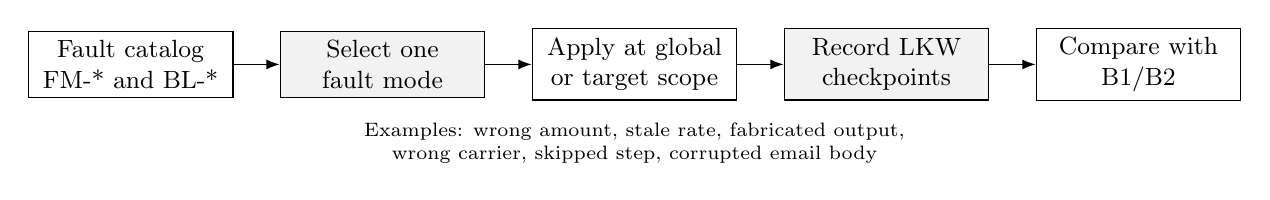
\begin{tikzpicture}[
      box/.style={draw,align=center,minimum width=2.6cm,minimum height=0.8cm,font=\small},
      note/.style={align=center,font=\scriptsize},
      >=Latex
]
\node[box,fill=white] (catalog) at (0,0) {Fault catalog\\FM-* and BL-*};
\node[box,fill=gray!10] (select) at (3.2,0) {Select one\\fault mode};
\node[box,fill=white] (inject) at (6.4,0) {Apply at global\\or target scope};
\node[box,fill=gray!10] (trace) at (9.6,0) {Record LKW\\checkpoints};
\node[box,fill=white] (compare) at (12.8,0) {Compare with\\B1/B2};
\draw[->] (catalog) -- (select);
\draw[->] (select) -- (inject);
\draw[->] (inject) -- (trace);
\draw[->] (trace) -- (compare);
\node[note] at (6.4,-1.0) {Examples: wrong amount, stale rate, fabricated output,\\wrong carrier, skipped step, corrupted email body};
\end{tikzpicture}}
\caption{Fault-injection workflow. Each B3 run activates one controlled fault
mode at its configured global or targeted scope, records the resulting LKW
trace, and evaluates the trace using fixed B1/B2 comparison relations.}
\Description{A five-step flow from the fault catalog through selecting one mode, applying its configured scope, recording LKW checkpoints, and comparing the trace with B1 and B2.}
\label{fig:fault-injection-simple}
\end{figure}

\begin{table*}[t]
\centering
\caption{Injection design, observation method, and interpretation for each
evaluated fault class.}
\label{tab:injection-design}
\begin{tabularx}{\textwidth}{lYYY}
\toprule
\textbf{Fault class} & \textbf{How we injected it} & \textbf{Observed by LKW} & \textbf{What the result says} \\
\midrule
FM-3.1 Premature termination
      & Return early before one or more required tool/service calls
      & Required checkpoints are absent from the B3 trace
      & LKW can detect structural workflow loss without semantic analysis \\
FM-1.2 Wrong action/routing
      & Swap the selected action, route, currency, carrier, or recipient before the tool call
      & Correct step sequence may remain, but the guarded route/action value differs from B1
      & Agent workflows need routing and parameter checks, not only step-count checks \\
FM-2.2 Hallucinated output
      & Replace a real tool/service result with a fabricated but plausible value
      & A checkpoint or handoff carries an invalid value; the intended internal checkpoint may also be missing
      & Value checks can expose a plausible output even when step evidence is incomplete \\
FM-2.5 Input ignored or replaced
      & Ignore or replace an input before use, such as an amount, query, or context
      & The guarded value differs at the first recorded consumption or output point
      & LKW localizes the first recorded effect of input corruption \\
BL-* Business fault
      & Target the owning agent with domain-specific corruption such as overcharge, stale rate, wrong email, or wrong quote
      & GB and RB checkpoints expose different guarded variables
      & Domain labels matter because business harm differs across e-commerce and shipping \\
\bottomrule
\end{tabularx}
\end{table*}

\subsection{Fault Metadata and AgentTracer Conversion}

The configured fault mode is experimental metadata that identifies the known
cause of a controlled run; it is not itself detection evidence. Detection comes
from the raw LKW observations: a required step is absent, or a guarded value
violates its fixed B1/B2 relation. Some harnesses also emit diagnostic flags,
but these flags are used for controlled classification and are not assumed to
be available in production.

After trace generation, an adapter packages the evidence into 67
AgentTracer-compatible trajectories. It reconstructs 65 single-agent
trajectories from the HITL classifications and B1 checkpoint values, adding
synthetic deviation markers at the known infection steps. It converts two
cross-agent trajectories from the measured propagation artifact. The adapter
also attaches ground-truth agent and step fields derived from the injection
setup. These files establish format and ground-truth coverage; they are not 67
independent executions, and no saved attribution-evaluation report establishes
attribution accuracy.

% =============================================================================
\section{Experimental Protocol}
\label{sec:protocol-diagrams}
% =============================================================================

The method is summarized by the system architecture in
Figure~\ref{fig:architecture-simple}, the injection workflow in
Figure~\ref{fig:fault-injection-simple}, and the testing protocol in
Figure~\ref{fig:testing-protocol-simple}. Detailed numeric evidence is reported
in the result tables.

\begin{figure*}[t]
\centering
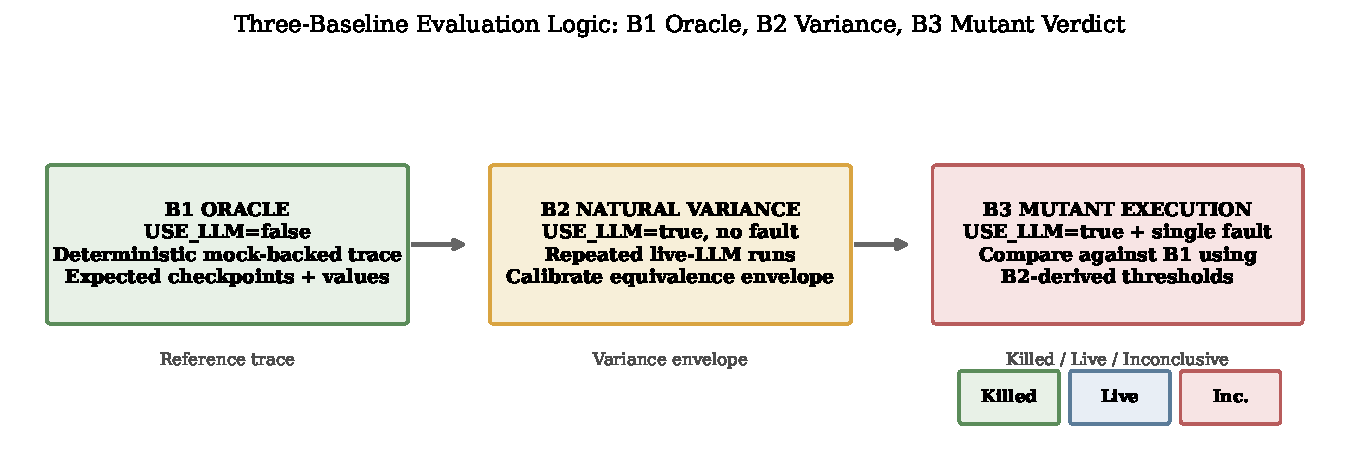
\includegraphics[width=0.9\textwidth]{fig_b123_protocol.pdf}
\caption{B1/B2/B3 testing workflow. B1 assembles expected checkpoint state,
B2 characterizes no-fault behavior on deterministic and live-LLM surfaces, and
B3 executes one configured fault mode. Fixed structural and field-level
relations produce the detection verdict and RIP explanation.}
\Description{The B1, B2, and B3 protocol: assemble expected checkpoint state, characterize no-fault behavior, execute one configured fault mode, compare traces, and produce a detection and RIP verdict.}
\label{fig:testing-protocol-simple}
\end{figure*}

The execution protocol has six steps:

\begin{enumerate}
  \item Assemble B1 field-level oracle values from six deterministic agent
        baselines and the selected no-fault shipping baseline.
  \item Run B2 without faults: repeat the six deterministic surfaces, exercise
        live-LLM shipping, and separately run the systematic live-LLM workflow.
  \item Run B3 with one fault mode at its declared global or targeted scope.
  \item Compare required steps and guarded values using the fixed B1/B2
        relations.
  \item Use RIP to report reachability, the first recorded infection when one
        can be localized, and downstream propagation.
  \item Classify each B3 run as detected, partially detected, false negative,
        or inconclusive. Separately classify eligible isolated traces into HITL
        tiers for manual review.
\end{enumerate}

% =============================================================================
\section{Evaluation Results by Research Question}
\label{sec:evaluation}
% =============================================================================

Each RQ is reported through its experiment design, measurement, and answer.
For run-level and mode-level proportions, we give numerator/denominator counts
and Wilson 95\% confidence intervals (CI). Location and depth fields are
descriptive outputs of the trace analysis, not estimates of localization or
attribution accuracy. The evidence scope is stated separately for each RQ.

\begin{table*}[t]
\centering
\caption{Research-question mapping between evidence, measurement, and confidence.
This table makes explicit how each evaluation result answers a specific RQ.}
\label{tab:rq-evidence-map}
\begin{tabularx}{\textwidth}{lYYY}
\toprule
\textbf{RQ} & \textbf{Primary evidence} & \textbf{Measurement} & \textbf{Confidence reporting} \\
\midrule
RQ1 Injection/reproducibility
      & Tables~\ref{tab:service-coverage-simple}, \ref{tab:b3-headline-simple}, \ref{tab:b3-fault-summary-simple}
      & Repeated campaign execution and run-level detection
      & Counts and Wilson 95\% CI; signature stability is evaluated only in RQ5 \\
RQ2 First infection location
      & Tables~\ref{tab:fault-lkw-ckpt}, \ref{tab:b3-fault-summary-simple}
      & Earliest deviating agent and expected checkpoint map
      & Descriptive consensus location; no localization-accuracy estimate \\
RQ3 Propagation depth
      & Table~\ref{tab:b3-fault-summary-simple} and two cross-agent chains
      & Later-deviation depth in B3 and boundary outcome in measured chains
      & Descriptive only; global FM injection prevents causal attribution of later deviations \\
RQ4 HITL classification
      & Table~\ref{tab:hitl-summary-simple}
      & Automatic detectability and HITL requirement across 48 injected cases
      & Counts and Wilson 95\% CI for campaign composition, not classifier accuracy \\
RQ5 Stability across runs
      & ShippingAgent stability artifact
      & Structural-fingerprint repeatability for 11 modes, three runs each
      & 11/11 with Wilson 95\% CI; ShippingAgent only \\
RQ6 Boundary recovery potential
      & Two measured cross-agent chains
      & Policy execution and HITL avoidance
      & 2/2 policies executed; 1/2 avoided HITL; feasibility evidence only \\
RQ7 Failure attribution
      & AgentTracer trajectory index
      & Conversion count and availability of ground-truth fields
      & Artifact count only; no attribution predictions were evaluated \\
\bottomrule
\end{tabularx}
\end{table*}

\begin{table}[t]
\centering
\caption{Complete targeted ten-fault B3 matrix by model configuration. Each
fault--configuration cell has three repetitions. TP means at least two compared
agents deviated; PTP means exactly one compared agent deviated. Both count as
detected; the rate excludes inconclusive runs. Wilson 95\% CIs use run-level
counts.}
\label{tab:b3-headline-simple}
\footnotesize
\begin{tabularx}{\columnwidth}{lrrrrY}
\toprule
\textbf{Config} & \textbf{TP} & \textbf{PTP} & \textbf{FN} & \textbf{INC} & \textbf{Detection (95\% CI)} \\
\midrule
3b, $t{=}0.7$ & 12 & 16 & 2 & 0 & 28/30 = 93.3\% [78.7, 98.2]\% \\
3b, $t{=}1.0$ & 11 & 12 & 5 & 2 & 23/28 = 82.1\% [64.4, 92.1]\% \\
\midrule
\textbf{Total} & \textbf{23} & \textbf{28} & \textbf{7} & \textbf{2} & \textbf{51/58 = 87.9\% [77.1, 94.0]\%} \\
\bottomrule
\end{tabularx}
\end{table}

The repository also contains lower-temperature summaries, but those campaigns
do not contain all ten current targeted faults and include earlier global
business-fault injections. They are excluded from the pooled estimate rather
than treated as missing or live mutants.

\begin{table*}[t]
\centering
\caption{Fault-by-fault evidence in the complete targeted matrix. Counts pool
the two model configurations and three repetitions per configuration. Detection
is $(\mathrm{TP}+\mathrm{PTP})/(\mathrm{TP}+\mathrm{PTP}+\mathrm{FN})$; INC is
reported separately. ``Earliest deviating agent'' follows workflow order.
``Max later dev.'' counts later deviating agents and is not necessarily causal
propagation.}
\label{tab:b3-fault-summary-simple}
\footnotesize
\begin{tabularx}{\textwidth}{lrrrrYcY}
\toprule
\textbf{Fault} & \textbf{TP} & \textbf{PTP} & \textbf{FN} & \textbf{INC} & \textbf{Earliest deviating agent} & \textbf{Max later dev.} & \textbf{Detection (95\% CI)} \\
\midrule
FM-3.1 Premature termination & 6 & 0 & 0 & 0 & ProductCatalogAgent (GB) & 5 & 6/6 = 100\% [61.0, 100]\% \\
FM-1.2 Wrong route/action    & 5 & 0 & 0 & 1 & ProductCatalogAgent (GB) & 5 & 5/5 = 100\% [56.6, 100]\% \\
FM-2.2 Hallucinated output   & 6 & 0 & 0 & 0 & ProductCatalogAgent (GB) & 4 & 6/6 = 100\% [61.0, 100]\% \\
FM-2.5 Value tampering       & 6 & 0 & 0 & 0 & ProductCatalogAgent (GB) & 3 & 6/6 = 100\% [61.0, 100]\% \\
BL-PRICE\_MANIP.             & 0 & 6 & 0 & 0 & ProductCatalogAgent (GB) & 0 & 6/6 = 100\% [61.0, 100]\% \\
BL-RATE\_MANIP.              & 0 & 6 & 0 & 0 & CurrencyAgent (GB)       & 0 & 6/6 = 100\% [61.0, 100]\% \\
BL-AMOUNT\_TAMP.             & 0 & 5 & 1 & 0 & PaymentAgent (GB)        & 0 & 5/6 = 83.3\% [43.6, 97.0]\% \\
BL-INVENTORY\_MISM.          & 0 & 5 & 1 & 0 & ShippingQuoteAgent (RB)  & 0 & 5/6 = 83.3\% [43.6, 97.0]\% \\
BL-SHIPMENT\_LOST            & 0 & 5 & 1 & 0 & ShipOrderAgent (RB)      & 0 & 5/6 = 83.3\% [43.6, 97.0]\% \\
BL-CORRUPTED\_BODY           & 0 & 1 & 4 & 1 & EmailServiceAgent (GB)   & 0 & 1/5 = 20.0\% [3.6, 62.4]\% \\
\bottomrule
\end{tabularx}
\end{table*}

\subsection{RQ1: Can faults be injected and reproduced?}

\textbf{Experiment design.} Activate one configured fault mode per B3 run and
repeat each fault--configuration cell three times. General FM modes are global;
business BL modes target their owning agent.

\textbf{Measurement.} Agent-role evidence coverage and the proportion of
conclusive B3 runs with at least one compared-agent deviation.

\textbf{Answer.} The configured modes were executed repeatedly, but
observability was not uniform. Table~\ref{tab:service-coverage-simple}
separates isolated harness coverage from systematic B3 participation. The
complete matrix covers product, currency, payment, email, shipping quote, and
ship order; recommendation, ad, and cart are not pooled into its estimate.
Among 58 conclusive runs, 51 exposed at least one deviation (87.9\%, Wilson
95\% CI [77.1, 94.0]\%); two additional runs were inconclusive. The observed
rate was 93.3\% at temperature 0.7 and 82.1\% at temperature 1.0. These counts
show repeatable campaign execution and measured detection, while uniform
signature reproducibility is assessed only for ShippingAgent in RQ5.
Primary evidence comes from Tables~\ref{tab:service-coverage-simple},
\ref{tab:b3-headline-simple}, and \ref{tab:b3-fault-summary-simple}; confidence
for the main detection proportion is reported as Wilson 95\% CI.

\subsection{RQ2: Where does failure first appear?}

\textbf{Experiment design.} For each B3 trace, identify the first recorded
checkpoint whose value or required-step status violates its B1/B2 relation.

\textbf{Measurement.} Earliest deviating agent in workflow order, supplemented
by the predeclared expected checkpoint map.

\textbf{Answer.} Structural evidence appears as a missing required checkpoint;
semantic evidence appears as a guarded-value deviation at a completed
checkpoint or handoff. Table~\ref{tab:fault-lkw-ckpt} gives the expected
field-level observation point, while Table~\ref{tab:b3-fault-summary-simple}
reports the earliest deviating agent summarized from B3. For the four global
FM modes, ProductCatalogAgent appears first because it is the first
service-facing agent in the fixed workflow and all agents receive the mode;
this is an observation location, not attribution to a unique fault origin.
The saved aggregate does not evaluate checkpoint-localization accuracy, and a
checkpoint can remain unlocalized when it is missing, as in Chain A.
Primary evidence comes from Tables~\ref{tab:fault-lkw-ckpt} and
\ref{tab:b3-fault-summary-simple}; per-fault CIs describe detection, not the
accuracy of the reported location.

\subsection{RQ3: How far do failures propagate?}

\textbf{Experiment design.} Record agents that deviate after the earliest B3
deviation, and separately execute two targeted cross-agent chains with a clean
downstream agent.

\textbf{Measurement.} B3 later-deviation depth and cross-agent boundary outcome.

\textbf{Answer.} The systematic B3 summaries record three to five later
deviating agents for the global FM modes. Because those modes are injected into
every agent, these counts cannot establish that the earliest agent caused the
later deviations. For targeted BL runs, non-target agents are skipped by the
oracle comparison, so a zero depth also does not prove absence of propagation.
Causal evidence comes from the two targeted chains: the corrupted payload
reached each downstream boundary, where recovery either blocked it or restored
validated context, leaving the downstream operation clean. The study therefore
demonstrates boundary reach and containment in two cases, not uncontrolled
end-to-end propagation. All B3 depth maxima are descriptive.

\subsection{RQ4: Which failures auto-resolve and which need HITL?}

\textbf{Experiment design.} Classify 48 injected isolated-agent traces using
their structural and diagnostic signatures; exclude six \texttt{NONE}
baselines.

\textbf{Measurement.} Automatic detectability, HITL requirement, and three
evidence tiers: structural, flag-detectable, and silent semantic.

\textbf{Answer.} All 48 injected cases are marked as requiring HITL in the saved
classification. Eight Tier~1 cases are also automatically detectable from
structural evidence; automatic detection does not mean automatic resolution.
The remaining 34 Tier~2 and 6 Tier~3 cases are not marked auto-detectable.
Tier~2 uses experimental diagnostic fields and would need equivalent runtime
predicates in production; Tier~3 requires semantic validation. The artifact
therefore answers detectability and review need, not which failures
auto-resolve. Recovery without HITL is evaluated separately in RQ6.

\begin{table}[t]
\centering
\caption{HITL tier evidence. Tier 1 is structural, Tier 2 is flag-detectable,
and Tier 3 is silent semantic. Proportions are reported for 48 injected cases
across six GB agents with Wilson 95\% CI. Six \texttt{NONE} baselines are
excluded.}
\label{tab:hitl-summary-simple}
\footnotesize
\begin{tabularx}{\columnwidth}{lrrYY}
\toprule
\textbf{Tier} & \textbf{Cases} & \textbf{Auto-detect?} & \textbf{Detection method} & \textbf{Share (95\% CI)} \\
\midrule
Tier 1 Structural & 8 & yes & Missing-step or depth difference & 16.7\% [8.7, 29.6]\% \\
Tier 2 Flag-detectable & 34 & no & Harness fields; runtime check needed & 70.8\% [56.8, 81.8]\% \\
Tier 3 Silent semantic & 6 & no & Semantic validation using B1/B2 relations & 12.5\% [5.9, 24.7]\% \\
\bottomrule
\end{tabularx}
\end{table}

Primary evidence comes from Table~\ref{tab:hitl-summary-simple}. The Wilson
intervals describe the tier shares in this finite campaign; they do not measure
classification accuracy.

\subsection{RQ5: Are observations stable across repeated runs?}

\textbf{Experiment design.} Repeat fault runs under controlled compute settings.

\textbf{Measurement.} Equality of infection point, reached-step sequence, and
propagation-depth field across three repetitions of each mode.

\textbf{Answer.} The stability artifact contains three repetitions for each of
11 ShippingAgent modes. All 11 structural fingerprints are identical across
their repetitions (100\%, Wilson 95\% CI [74.1, 100.0]\%). The fingerprint does
not compare all guarded payload values, and this result does not establish
system-wide or semantic-value stability.

\subsection{RQ6: Can boundary recovery reduce HITL burden?}

\textbf{Experiment design.} Apply simple boundary policies such as schema,
range, and consistency checks at agent-to-agent handoff points.

\textbf{Measurement.} Whether the boundary detects the violation, executes its
specified policy, and avoids HITL.

\textbf{Answer.} Chain A changed the expected amount from 9 to 1337 units
(14,755.6\% difference); the payment boundary blocked the charge and requested
HITL. Chain B removed the expected catalog product ID; the recommendation
boundary restored the last-known-good ID and continued without HITL. Both
boundaries detected the violation and executed their specified policy (2/2,
Wilson 95\% CI [34.2, 100.0]\%). Only one chain avoided HITL (1/2, 50.0\%,
Wilson 95\% CI [9.5, 90.5]\%). These are feasibility results for two predefined
policies, not a general reduction rate.

\subsection{RQ7: Can failure attribution identify the responsible agent?}

\textbf{Experiment design.} Convert existing HITL, stability, oracle, and
cross-agent artifacts into AgentTracer-compatible trajectory files with known
source-agent metadata.

\textbf{Measurement.} Number of converted trajectories and presence of
ground-truth fields. No attributor predictions are measured.

\textbf{Answer.} The adapter produced 65 reconstructed single-agent and 2
converted cross-agent trajectories, for 67 files total. Ground-truth agent and
step fields are present in the schema, but values can be null for baselines or
unlocalized cases such as Chain A. The single-agent files use B1 values and
synthetic deviation markers derived from HITL classifications; they are not
independent fault executions. No saved attribution-evaluation report contains
predictions to compare with this ground truth, so RQ7 remains unanswered as an
accuracy question. The current result establishes only conversion readiness.

\clearpage

% =============================================================================
\section{Discussion}
% =============================================================================

The main lesson is that agentic microservice testing must observe data values,
not only task completion. A final answer can look successful even when the
agent has already corrupted the amount, product, quote, or recipient. LKW
checkpoints make these hidden values visible. RIP then explains whether the
fault was merely reached, whether it infected state, and whether it propagated
to business harm.

The second lesson is that B1 must be clearly understood as the oracle. Without
B1, there is no definition of correctness at the checkpoint. Without B2, normal
LLM variance may be mistaken for a fault. Without B3, the checkpoint design is
not stress-tested against controlled failures.

The third lesson is that GB and RB should not be merged casually. GB faults
mostly concern e-commerce data such as prices, products, payments, and emails.
RB faults concern shipping decisions such as carrier, quote, delivery window,
tracking, and escalation. Keeping these domains separate lets us observe domain
drift instead of hiding it.

% =============================================================================
\section{Threats to Validity}
% =============================================================================

\textbf{Live-LLM variance.} LLM execution is nondeterministic even with fixed
settings, so B2 is required before judging B3.

\textbf{Benchmark scope.} The current evidence is strongest for the checkout
and shipping workflows studied here. Other domains may require different LKW
checkpoint variables.

\textbf{Unequal campaign coverage.} Only the temperature-0.7 and
temperature-1.0 configurations contain the complete ten-fault targeted matrix.
Lower-temperature summaries are retained as artifacts but excluded from the
pooled B3 estimate. Each complete cell has only three repetitions, producing
wide per-fault confidence intervals.

\textbf{Controlled service responses.} Systematic helpers use Ollama for agent
decisions and mock clients for service responses. The results establish fault
observability under controlled interfaces, not resilience of a fully deployed
gRPC system.

\textbf{Attribution and stability scope.} AgentTracer conversion is complete
for 67 trajectories, but attribution accuracy has not been evaluated in a
saved report. The repeated-run stability result covers ShippingAgent only.

\textbf{HITL automation.} HITL tiers are identifiable from traces, but the
current workflow still depends on manual trace inspection for final judgments.
An automated verifier agent is future work.

\textbf{Mutation terminology.} We use mutant-operator language only as a
convenient label for injected controlled faults. The central contribution is
not test-suite mutation adequacy; it is LKW/RIP fault observability.

% =============================================================================
\section{Conclusion}
% =============================================================================

This paper argues for a checkpoint-centered view of agentic
microservice reliability. B1 defines correct checkpoint values, B2 defines
normal LLM variance, and B3 injects controlled faults to test whether LKW/RIP
can expose reachability, infection, and propagation. The important result is
not a standalone mutation score. The important result is that semantic faults
can pass through successful-looking agent workflows unless the system validates
data at the checkpoints where one agent's output becomes another agent's input.

% =============================================================================
\section*{Acknowledgment}
% =============================================================================

The author thanks the project supervisors and team collaborators for guidance
on scenario design, benchmark sequencing, and research-question framing.

% =============================================================================
\bibliographystyle{ACM-Reference-Format}
\begin{thebibliography}{00}

\bibitem{lkw}
J.~W.~Laski and B.~Korel, ``A data flow oriented program testing strategy,''
\textit{IEEE Trans.\ Softw.\ Eng.}, vol.~9, no.~3, pp.~347--354, 1983.

\bibitem{rapps-weyuker}
S.~Rapps and E.~J.~Weyuker, ``Selecting software test data using data flow
information,'' \textit{IEEE Trans.\ Softw.\ Eng.}, vol.~11, no.~4,
pp.~367--375, 1985.

\bibitem{chaosengineering}
P.~Basiri \textit{et al.}, ``Chaos engineering,''
\textit{IEEE Software}, vol.~33, no.~3, pp.~35--41, 2016.

\bibitem{microservicefi}
B.~Canizo \textit{et al.}, ``Fault injection in microservice-based systems:
A systematic review,'' \textit{J.\ Syst.\ Softw.}, vol.~195, 2023.

\bibitem{istio}
Istio Contributors, ``Traffic Management: Fault Injection,''
in \textit{Istio Documentation}, 2023.

\bibitem{google-ob}
Google LLC, ``Microservices Demo: Online Boutique,'' GitHub repository,
\url{https://github.com/GoogleCloudPlatform/microservices-demo}, 2024.

\bibitem{react}
S.~Yao, J.~Zhao, D.~Yu, N.~Du, I.~Shafran, K.~Narasimhan, and Y.~Cao,
``ReAct: Synergizing Reasoning and Acting in Language Models,''
in \textit{Proc.\ ICLR}, 2023.

\bibitem{agentbench}
X.~Liu \textit{et al.}, ``AgentBench: Evaluating LLMs as agents,''
in \textit{Proc.\ ICLR}, 2024.

\bibitem{toolbench}
Y.~Qin \textit{et al.}, ``ToolLLM: Facilitating large language models to
master real-world APIs,'' in \textit{Proc.\ ICLR}, 2024.

\bibitem{langgraph}
LangChain Contributors, ``LangGraph: Build stateful, multi-actor applications
with LLMs,'' LangChain GitHub, 2024.

\bibitem{autogen}
Q.~Wu \textit{et al.}, ``AutoGen: Enabling next-gen LLM applications via
multi-agent conversation,'' in \textit{Proc.\ COLM}, 2024.

\bibitem{nemoguar}
T.~Rebedea \textit{et al.}, ``NeMo Guardrails: A toolkit for controllable and
safe LLM applications with programmable rails,''
in \textit{Proc.\ EMNLP (Demo)}, 2023.

\bibitem{llmguardrails}
S.~Dong \textit{et al.}, ``Building guardrails for large language models,''
\textit{arXiv:2402.01822}, 2024.

\end{thebibliography}

\end{document}
